\documentclass[12pt]{article}
\usepackage[utf8]{inputenc}
\usepackage{parskip}
\usepackage{tabularx}
\usepackage{syntax} % grammar format
% \usepackage{markdown} % inline mark down
\usepackage[color, leftbars]{changebar}
\usepackage{subcaption}

%%%%%%%%%%%%%%%%%%%%%%%%%%%%%%%%%%%%%%%%%%%%%%%%%%%%%%%%%%%%%%%%%%%%%%%%
% Reduce margin
%
% \addtolength{\oddsidemargin}{-.85in}
% \addtolength{\evensidemargin}{-.85in}
% \addtolength{\textwidth}{1in}

% \addtolength{\topmargin}{-.85in}
% \addtolength{\textheight}{1in}

% Reduce margin
%
\addtolength{\oddsidemargin}{-.85in}
\addtolength{\evensidemargin}{-.85in}
\addtolength{\textwidth}{1in}

\addtolength{\topmargin}{-.90in}
\addtolength{\textheight}{1.75in}


% Page format commands:
% Override normal article margins,
% making the margins smaller
% \setlength{\textwidth}{6.5in}
% \setlength{\textheight}{9in}
% \setlength{\oddsidemargin}{0in}
% \setlength{\evensidemargin}{0in}
% \setlength{\topmargin}{-0.5in}

\setlength{\parindent}{0pt}

\setlength{\grammarparsep}{20pt plus 1pt minus 1pt} % increase separation between rules
\setlength{\grammarindent}{10em} % increase separation between LHS/RHS 
%%%%%%%%%%%%%%%%%%%%%%%%%%%%%%%%%%%%%%%%%%%%%%%%%%%%%%%%%%%%%%%%%%%%%%%%


%%%%%%%%%%%%%%%%%%%%%%%%%%%%%%%%%%%%%%%%%%%%%%%%%%%%%%%%%%%%%%%%%%%%%%%%
% Math Symbols
\usepackage{mathtools}
\usepackage{amssymb}
% \usepackage{epsfig}
\usepackage{amsmath,amsthm}
\usepackage{amscd,amsxtra,latexsym}


% add floor and ceiling symbol. Usage: \ceil*{}, \floor*{}
% \DeclarePairedDelimiter\ceil{\lceil}{\rceil}
% \DeclarePairedDelimiter\floor{\lfloor}{\rfloor}

% multiset \langle ... \rangle
\def\multiset#1#2{\ensuremath{\left(\kern-.3em\left(\genfrac{}{}{0pt}{}{#1}{#2}\right)\kern-.3em\right)}}



%%%%%%%%%%%%%%%%%%%%%%%%%%%%%%%%%%%%%%%%%%%%%%%%%%%%%%%%%%%%%%%%%%%%%%%%


%%%%%%%%%%%%%%%%%%%%%%%%%%%%%%%%%%%%%%%%%%%%%%%%%%%%%%%%%%%%%%%%%%%%%%%%
% Code Sample Styling

% use \lstinline! (inline text) ! or \begin{lstlisting} text block \end{lstlisting}
\usepackage{listings}

\usepackage{color}
\definecolor{light-gray}{gray}{0.97} % shade of grey
\definecolor{dkgreen}{rgb}{0,0.6,0}
\definecolor{gray}{rgb}{0.5,0.5,0.5}
\definecolor{mauve}{rgb}{0.58,0,0.82}

% \begin{lstlisting}[...] ... \end{lstlisting}
\lstset{frame=none,
    language=[Objective]Caml,
    aboveskip=3mm,
    belowskip=3mm,
    stepnumber=0, % set to 0 if you don't like line nums
    showstringspaces=false,
    columns=flexible,
    basicstyle={\small\ttfamily},
    numbers=left,
    numberstyle=\color{black},
    keywordstyle=\color{blue},
    commentstyle=\color{dkgreen},
    stringstyle=\color{mauve},
    backgroundcolor=\color{light-gray},
    breaklines=true,
    breakatwhitespace=false,
    tabsize=2
}



%%%%%%%%%%%%%%%%%%%%%%%%%%%%%%%%%%%%%%%%%%%%%%%%%%%%%%%%%%%%%%%%%%%%%%%%


%%%%%%%%%%%%%%%%%%%%%%%%%%%%%%%%%%%%%%%%%%%%%%%%%%%%%%%%%%%%%%%%%%%%%%%%
\usepackage{xcolor}
%% https://tex.stackexchange.com/questions/401750/quick-and-short-command-for-coloring-one-word
\newcommand\shorthandon{\catcode`@=\active \catcode`^=\active \catcode`*=\active }
\newcommand\shorthandoff{\catcode`@=12 \catcode`^=7 \catcode`*=12 }
\shorthandon
\def@#1@{\textcolor{red}{#1}}%
\def^#1^{\textcolor{blue}{#1}}%
\def*#1{\string#1}
\shorthandoff
%% useage: \textcolor{red}{text here}
% \shorthandon
% This is a @test@ of the ^emergency^ bro*@dcast system.
% \shorthandoff
%%%%%%%%%%%%%%%%%%%%%%%%%%%%%%%%%%%%%%%%%%%%%%%%%%%%%%%%%%%%%%%%%%%%%%%%


%%%%%%%%%%%%%%%%%%%%%%%%%%%%%%%%%%%%%%%%%%%%%%%%%%%%%%%%%%%%%%%%%%%%%%%%
% Misc
\usepackage{graphicx} % graphics
\usepackage{enumitem} % listing style (bullet lists)

% below helps with trying to get figures in a row
% \usepackage{caption}
% \usepackage{subcaption}

% hyperlink styling
% use \href{} and \url{}, and colors table of contents links
% use \href{} and \url{}
% \label{sec:name}
% \hyperref[label]{text}
\usepackage{hyperref}
\hypersetup{
    colorlinks=true,
    linkcolor=blue, % was previously black
    filecolor=magenta,
    urlcolor=blue,
    pdftitle={groot LRM}
}
\urlstyle{same}

% A command for primes (')
\newcommand{\p}%
    {\ensuremath{^{\prime}}}

% a command for double primes ('')
\newcommand{\pp}%
    {\ensuremath{^{\prime \prime}}}

% A command for the Kleene star
\newcommand{\str}%
    {\ensuremath{^{\star}}}

% a command for the double star
\newcommand{\sstr}%
    {\ensuremath{^{\star\star}}}
%%%%%%%%%%%%%%%%%%%%%%%%%%%%%%%%%%%%%%%%%%%%%%%%%%%%%%%%%%%%%%%%%%%%%%%%



\begin{document} 
\title{(g)ROOT \\ Final Report}

\begin{figure}
    \centering
    
\includegraphics{images/babygroot.PNG}
\end{figure}

\author{Samuel Russo \quad Amy Bui \quad Eliza Encherman \\ Zachary Goldstein \quad Nickolas Gravel}
\date{\today}
\maketitle

    \pagebreak
    %%%%%%%%%%%%%%%%%%%%%%%%%%%%%%%%%%%%%%%%%%%%%%%%%%%%%%%%%%%%%%%%%%%%%%%%
    % Table of Contents
    \setcounter{tocdepth}{3}
    \tableofcontents
    \pagebreak 
    %%%%%%%%%%%%%%%%%%%%%%%%%%%%%%%%%%%%%%%%%%%%%%%%%%%%%%%%%%%%%%%%%%%%%%%%



%%%%%%%%%%%%%%%%%%%%%%%%%%%%%%%%%%%%%%%%%%%%%%%%%%%%%%%%%%%%%%%%%%%%%%%%%%%%%%%
%%%%%%%%%%%%%%%%%%%%%%%%%%%%%%%%%%%%%%%%%%%%%%%%%%%%%%%%%%%%%%%%%%%%%%%%%%%%%%%
%%%%%%%%%%%%%%%%%%%%%%%%%%%%%%%%% ACK %%%%%%%%%%%%%%%%%%%%%%%%%%%%%%%%%%%%%%%
%%%%%%%%%%%%%%%%%%%%%%%%%%%%%%%%%%%%%%%%%%%%%%%%%%%%%%%%%%%%%%%%%%%%%%%%%%%%%%%
%%%%%%%%%%%%%%%%%%%%%%%%%%%%%%%%%%%%%%%%%%%%%%%%%%%%%%%%%%%%%%%%%%%%%%%%%%%%%%%
\section{Acknowledgments}
\label{sec:ACK}

  Project Mentor: Mert Erden

  Professor: Richard Townsend 

\section{Resources}
\label{sec:resource}
  Implementing functional languages: a tutorial. Simon Peyton Jones, David R Lester. Prentice Hall, 1992.

  Modern Compiler Implementation in ML. Andrew W. Appel. Cambridge University Press, 2004.

  Compilers: Principles, Techniques, and Tools, 2nd Edition. Alfred V. Aho, Monica S. Lam, Ravi Sethi, Jeffrey D. Ullman. Addison-Wesley, 2006.

  Engineering a Compiler, 2th Edition. Keith D. Cooper and Linda Torczon. Morgan Kauf-mann, 2012.

  \href{https://v2.ocaml.org/manual/index.html}{OCaml Manual}

%%%%%%%%%%%%%%%%%%%%%%%%%%%%%%%%%%%%%%%%%%%%%%%%%%%%%%%%%%%%%%%%%%%%%%%%%%%%%%%
%%%%%%%%%%%%%%%%%%%%%%%%%%%%%%%%%%%%%%%%%%%%%%%%%%%%%%%%%%%%%%%%%%%%%%%%%%%%%%%
%%%%%%%%%%%%%%%%%%%%%%%%%%%%%%%%% ACK %%%%%%%%%%%%%%%%%%%%%%%%%%%%%%%%%%%%%%%
%%%%%%%%%%%%%%%%%%%%%%%%%%%%%%%%%%%%%%%%%%%%%%%%%%%%%%%%%%%%%%%%%%%%%%%%%%%%%%%
%%%%%%%%%%%%%%%%%%%%%%%%%%%%%%%%%%%%%%%%%%%%%%%%%%%%%%%%%%%%%%%%%%%%%%%%%%%%%%%





%%%%%%%%%%%%%%%%%%%%%%%%%%%%%%%%%%%%%%%%%%%%%%%%%%%%%%%%%%%%%%%%%%%%%%%%%%%%%%%
%%%%%%%%%%%%%%%%%%%%%%%%%%%%%%%%%%%%%%%%%%%%%%%%%%%%%%%%%%%%%%%%%%%%%%%%%%%%%%%
%%%%%%%%%%%%%%%%%%%%%%%%%%%%%%%%% INTRO %%%%%%%%%%%%%%%%%%%%%%%%%%%%%%%%%%%%%%%
%%%%%%%%%%%%%%%%%%%%%%%%%%%%%%%%%%%%%%%%%%%%%%%%%%%%%%%%%%%%%%%%%%%%%%%%%%%%%%%
%%%%%%%%%%%%%%%%%%%%%%%%%%%%%%%%%%%%%%%%%%%%%%%%%%%%%%%%%%%%%%%%%%%%%%%%%%%%%%%
\section{Introduction}
\label{sec:INTRO}

  g(ROOT) is a general-purpose functional programming language, with a pared-down and minimalistic syntax that makes it useful for educational purposes, such as transitioning imperative programmers to functional languages. The language has a LISP-like syntax and offers lambda expressions, higher-order functions, inferred types, and allows variable redefinitions. 

  g(ROOT) utilizes the Hindley-Milner algorithm in order to infer the types of expressions, as well as typing and variable environments in order to accomplish closure conversion to resolve lambda expressions (closures use the original values of any free variables at the time the closure was created, rather than using the most recent values of any free variables when the closure is used).
  
  The project originally set out to give the language a built-in n-ary tree data structure as a primitive type. This is where the name and mascot "groot" originates. However, with the challenges of compiling seemingly inherent functional language features and the time constraints, trees are left as a future feature to be implemented. 

  This document will provide an in-depth language reference manual for g(ROOT), a language tutorial, and details of our implementations and key takeaways from this project. 

\pagebreak
%%%%%%%%%%%%%%%%%%%%%%%%%%%%%%%%%%%%%%%%%%%%%%%%%%%%%%%%%%%%%%%%%%%%%%%%%%%%%%%
%%%%%%%%%%%%%%%%%%%%%%%%%%%%%%%%%%%%%%%%%%%%%%%%%%%%%%%%%%%%%%%%%%%%%%%%%%%%%%%
%%%%%%%%%%%%%%%%%%%%%%%%%%%%%%%%% INTRO %%%%%%%%%%%%%%%%%%%%%%%%%%%%%%%%%%%%%%%
%%%%%%%%%%%%%%%%%%%%%%%%%%%%%%%%%%%%%%%%%%%%%%%%%%%%%%%%%%%%%%%%%%%%%%%%%%%%%%%
%%%%%%%%%%%%%%%%%%%%%%%%%%%%%%%%%%%%%%%%%%%%%%%%%%%%%%%%%%%%%%%%%%%%%%%%%%%%%%%








%%%%%%%%%%%%%%%%%%%%%%%%%%%%%%%%%%%%%%%%%%%%%%%%%%%%%%%%%%%%%%%%%%%%%%%%%%%%%%%
%%%%%%%%%%%%%%%%%%%%%%%%%%%%%%%%%%%%%%%%%%%%%%%%%%%%%%%%%%%%%%%%%%%%%%%%%%%%%%%
%%%%%%%%%%%%%%%%%%%%%%%%%%%%%%%% TUTORIAL %%%%%%%%%%%%%%%%%%%%%%%%%%%%%%%%%%%%%
%%%%%%%%%%%%%%%%%%%%%%%%%%%%%%%%%%%%%%%%%%%%%%%%%%%%%%%%%%%%%%%%%%%%%%%%%%%%%%%
%%%%%%%%%%%%%%%%%%%%%%%%%%%%%%%%%%%%%%%%%%%%%%%%%%%%%%%%%%%%%%%%%%%%%%%%%%%%%%%
\section{Language Tutorial}
\label{sec:TUTORIAL}

\pagebreak
%%%%%%%%%%%%%%%%%%%%%%%%%%%%%%%%%%%%%%%%%%%%%%%%%%%%%%%%%%%%%%%%%%%%%%%%%%%%%%%
%%%%%%%%%%%%%%%%%%%%%%%%%%%%%%%%%%%%%%%%%%%%%%%%%%%%%%%%%%%%%%%%%%%%%%%%%%%%%%%
%%%%%%%%%%%%%%%%%%%%%%%%%%%%%%%% TUTORIAL %%%%%%%%%%%%%%%%%%%%%%%%%%%%%%%%%%%%%
%%%%%%%%%%%%%%%%%%%%%%%%%%%%%%%%%%%%%%%%%%%%%%%%%%%%%%%%%%%%%%%%%%%%%%%%%%%%%%%
%%%%%%%%%%%%%%%%%%%%%%%%%%%%%%%%%%%%%%%%%%%%%%%%%%%%%%%%%%%%%%%%%%%%%%%%%%%%%%%









%%%%%%%%%%%%%%%%%%%%%%%%%%%%%%%%%%%%%%%%%%%%%%%%%%%%%%%%%%%%%%%%%%%%%%%%%%%%%%%
%%%%%%%%%%%%%%%%%%%%%%%%%%%%%%%%%%%%%%%%%%%%%%%%%%%%%%%%%%%%%%%%%%%%%%%%%%%%%%%
%%%%%%%%%%%%%%%%%%%%%%%%%%%%%%%%%%% LRM %%%%%%%%%%%%%%%%%%%%%%%%%%%%%%%%%%%%%%%
%%%%%%%%%%%%%%%%%%%%%%%%%%%%%%%%%%%%%%%%%%%%%%%%%%%%%%%%%%%%%%%%%%%%%%%%%%%%%%%
%%%%%%%%%%%%%%%%%%%%%%%%%%%%%%%%%%%%%%%%%%%%%%%%%%%%%%%%%%%%%%%%%%%%%%%%%%%%%%%

%% LRM OUTLINE STARTS HERE
%%%%%%%%%%%%%%%%%%%%%%%%%%%%%%%%%%%%%%%%%%%%%%%%%%%%%%%%%%%%%%%%%%%%%%%%
\section{Language Reference Manual}
\label{sec:LRM}
    % \subsection{Intro}
    % \label{sec:lrmintro}

    % At its core, (g)ROOT is a general-purpose functional programming language. Its syntax stems from functional languages such as Scheme and other languages rooted in the Lisp family of programming languages. What sets Groot apart from other programming languages is its native employment of trees.

    % Trees are a widely-used, abstract data type that represents a hierarchical branching
    % structure, with a root value and subtrees of children. In many general-purpose
    % programming languages, trees are not a built-in feature. This forces the
    % programmer to implement them from the ground up, which can be a tedious process
    % for many beginner to intermediate programmers. Groot's built-in tree syntax
    % abstracts this logic away from the programmer, significantly reducing the
    % complexity inherent to tree development.

    % In the Groot programming language, trees are a primitive, immutable type
    % consisting of an element, sibling and child or a \textit{leaf}, a value
    % representing an empty tree. This allows programmers to easily pass trees between
    % functions, akin to passing lists in Lisp-style programming languages. Built-in
    % functions are also supplied to accomplish many common tree operations. These
    % language features alleviate the burden of implementing, operating, and
    % maintaining a tree data structure from the programmer, allowing them to focus on
    % solving more complex problems.


        \subsection{How to read manual}
        The syntax of the language will be given in BNF-like notation. Non-terminal symbol will be in italic font \emph{like-this}, square brackets [ … ] denote optional components, curly braces \{ … \} denote zero or more repetitions of the enclosed component,  and parentheses ( … ) denote a grouping. Note the font, as \texttt{[ ... ]} and \texttt{( ... )} are syntax requirements later in the manual.

    \pagebreak
    %% End of Introduction %%%%%%%%%%%%%%%%%%%%%%%%%%%%%%%%%%%%%%%%%%%


    %%%%%%%%%%%%%%%%%%%%%%%%%%%%%%%%%%%%%%%%%%%%%%%%%%%%%%%%%%%%%%%%%%%%%%%%
    \subsection{Lexical Convention}
    \label{sec:lexcon}
        
        \subsubsection{Blanks} %%%
        The following characters are considered as \textbf{blanks}: space, horizontal tab (`\texttt{\textbackslash t}'), newline character (`\texttt{\textbackslash n}'), and carriage return (`\texttt{\textbackslash r}'). 

        Blanks separate adjacent identifiers, literals, expressions, and keywords. They are otherwise ignored.
        %%%%%%%%%%%%%%%%%%%%%%%%%%%%%%%%%%%%%%%%%%%%%%%%%%%%%%%%%%%%%%%%%%%%%%%%

        \subsubsection{Comments}
        Comments are introduced with two adjact characters \texttt{(;} and terminated by two adjacent characters \texttt{;)}. Nested comments are currently not allowed. Multiline comments are allowed.\\

% \hspace{1cm}\begin{minipage}[h]{1\textwidth}
\cbcolor{dkgreen}
\cbstart
\begin{lstlisting}
(; This is a comment. ;)

(; This is a 
   multi-lined comment. ;)
\end{lstlisting}
\cbend
% \end{minipage}
        %%%%%%%%%%%%%%%%%%%%%%%%%%%%%%%%%%%%%%%%%%%%%%%%%%%%%%%%%%%%%%%%%%%%%%%%

        \subsubsection{Identifiers}
        \label{subsec:id}
        Identifiers are sequences of letters, digits, and ASCII characters, starting with a letter. Letters consist of the 26 lowercase and 26 uppercase characters from the ASCII set. Identifiers may not start with an underscore character, and may not be any of the \hyperref[subsec:key]{reserved character sequences}. 

        \hspace{1cm}\begin{minipage}[h]{1\textwidth}
        \begin{grammar}
            <ident> ::= $letter$\ ( $letter$ | $digit$ | \_ \ )
            
            <letter> ::= \texttt{a...z\ |\ A...Z }

            <digit> ::= \texttt{0...9 }
        \end{grammar}
        \end{minipage}
        %%%%%%%%%%%%%%%%%%%%%%%%%%%%%%%%%%%%%%%%%%%%%%%%%%%%%%%%%%%%%%%%%%%%%%%%


        \subsubsection{Integer Literals}
        \label{subsec:intlit}
        An integer literal is a decimal, represented by a sequence of one or more digits, optionally preceded by a minus sign. 

            \hspace{1cm}\begin{minipage}[h]{1\textwidth}
            \begin{grammar}
                <integer-literal> ::= [\ -\ ] $digit$ \big\{$digit$\big\}
    
                <digit> ::= \texttt{0...9 }
            \end{grammar}
            \end{minipage}
        %%%%%%%%%%%%%%%%%%%%%%%%%%%%%%%%%%%%%%%%%%%%%%%%%%%%%%%%%%%%%%%%%%%%%%%%

        \subsubsection{Boolean Literals}
        \label{subsec:boollit}
        Boolean literals are represented by two adjacent characters; the first is the octothorp character (\texttt{\#}), and it is immediately followed by either the \texttt{t} or the \texttt{f} character. 

            \hspace{1cm}\begin{minipage}[h]{1\textwidth}
            \begin{grammar}
                <boolean-literal> ::= \texttt{\#} (\ \texttt{t} |\ \texttt{f}\ )
            \end{grammar}
            \end{minipage}
        %%%%%%%%%%%%%%%%%%%%%%%%%%%%%%%%%%%%%%%%%%%%%%%%%%%%%%%%%%%%%%%%%%%%%%%%

        \subsubsection{Character Literals}
        \label{subsec:charlit}
        Character literals are a single character enclosed by two \textsf{'} (single-quote) characters.

        %%%%%%%%%%%%%%%%%%%%%%%%%%%%%%%%%%%%%%%%%%%%%%%%%%%%%%%%%%%%%%%%%%%%%%%%

        \subsubsection{Operators}
        \label{subsec:op}
        All of the following operators are prefix characters or prefixed characters read as single token. Binary operators are expected to be followed by two expressions, unary operators are expected to be followed by one expression. 

        \hspace{1cm}\begin{minipage}[h]{1\textwidth}
            \begin{grammar}

                <operator> ::= (\ \emph{unary-operator} |\ \emph{binary-operator}\ )

                <unary-operator> ::= \texttt{!} |\ \texttt{-}

                <binary-operator> ::= \ \texttt{+\ |\ -\ |\ *\ |\ /\ |\ mod }
                \alt\texttt{==\ |\ \textless\ |\ \textgreater\ |\ $\leq$ |\ $\geq$\ |\ != }
                \alt\texttt{\&\&\ |\ \textcolor{red}{||} }

            \end{grammar}
            \end{minipage}

        \subsection{Keywords}
        \label{subsec:key}
        The below identifiers are reserved keywords and cannot be used except in their capacity as reserve keywords: \\

\cbcolor{dkgreen}
\cbstart
\begin{lstlisting}
if      val         let
leaf    elm         tree
cld     sib         lambda
\end{lstlisting}
\cbend

        The following character sequence are also keywords: \\

\cbcolor{dkgreen}
\cbstart
\begin{lstlisting}
==      +       &&      >       '
!=      -       ||      mod     #t
<=      *       !       (       #f
>=      /       <       )       anon
\end{lstlisting}
\cbend

        \subsubsection{Syntax}
        \label{subsec:syn}

        See \hyperref[sec:expr]{Definitions and Expression} for concrete syntax for each definition and expressions, with examples.

    \pagebreak
    %% End of Lexical Convention %%%%%%%%%%%%%%%%%%%%%%%%%%%%%%%%%%%%%%%%%%%


    %%%%%%%%%%%%%%%%%%%%%%%%%%%%%%%%%%%%%%%%%%%%%%%%%%%%%%%%%%%%%%%%%%%%%%%%
    \subsection{Values}
    \label{sec:values}

    \paragraph{Base Values}

            \subsubsection{Integer numbers}
            Integer values are integer numbers in range from $-2^{32}$ to $2^{32} - 1$, similar to LLVM's integers, and may support a wider range of integer values on other machines, such as $-2^{64}$ to $2^{64} - 1$ on a 64-bit machine.

            \subsubsection{Boolean values}
            Booleans have two values. \texttt{\#t} evaluates to the boolean value \texttt{true}, and \texttt{\#f} evaluates to the boolean value \texttt{false}.

            \subsubsection{Characters}
            Character values are 8-bit integers between 0 and 255, and follow ASCII standard.

        \subsubsection{Functions}
        Functional values are mappings from values to value.

        % \subsection{Leaf}

        \subsubsection{N-Ary Tree Compound Type}
        A core feature of (g)ROOT is its n-ary tree compound value type. Every tree value consists of three components: an element, it's right-immediate sibling, and it's first child. This allows for the convenient implementation of robust recursive algorithms with an arbitrary branching factor.

        Every tree value in (g)ROOT may be either a full tree instance with an element, sibling, and child, or a leaf. The leaf value in (g)ROOT represents the nullary, or empty, tree.

        The tree type in (g)ROOT is modeled after a left-child right-sibling binary tree, where each node contains a reference to its first child and reference to its next sibling. This allows each node in (g)ROOT to have any number of children, while constraining the maximum number of fields per tree instance to three (element, sibling, and child).

        The tree type is very similar in usage to the one-dimensional list type present in many other functional languages, but enforces two additional invariants that empower programmers to shoot themselves in their foot less often.

        \begin{enumerate}
            \item The element of a tree instance may not be itself a tree. An element may be a value of any other type. This enforces a consistent structure among all trees that could be created in (g)ROOT.
            
            \textbf{Note}: it is possible to circumvent this requirement by wrapping a tree instance in a no-args lambda closure. This is a reasonable means of achieving nested data structures as it prevents the accidental creation of nested values; programmers who wrap tree instances in lambda closures likely did so with intention.


            \item Every tree node must have a single immediate sibling and a single immediate child. This forces programmers to think in a purely recursive manner about their solutions.
            
            Trees may be conveniently constructed in-place using the following construction syntax:\\

\cbcolor{dkgreen}
\cbstart
\begin{lstlisting}
'(value sibling-tree child-tree)
\end{lstlisting}
\cbend

For example:\\

\cbcolor{dkgreen}
\cbstart
\begin{lstlisting}
'(0 leaf (1 (2  (3 leaf leaf) (4 (5 (6 (leaf leaf)) leaf))) (7 (8 leaf leaf) (9 (10 leaf leaf) leaf))))
\end{lstlisting}
\cbend

represents the following tree (as drawn in normal binary tree form):
        \begin{figure}[h]
            \centering
            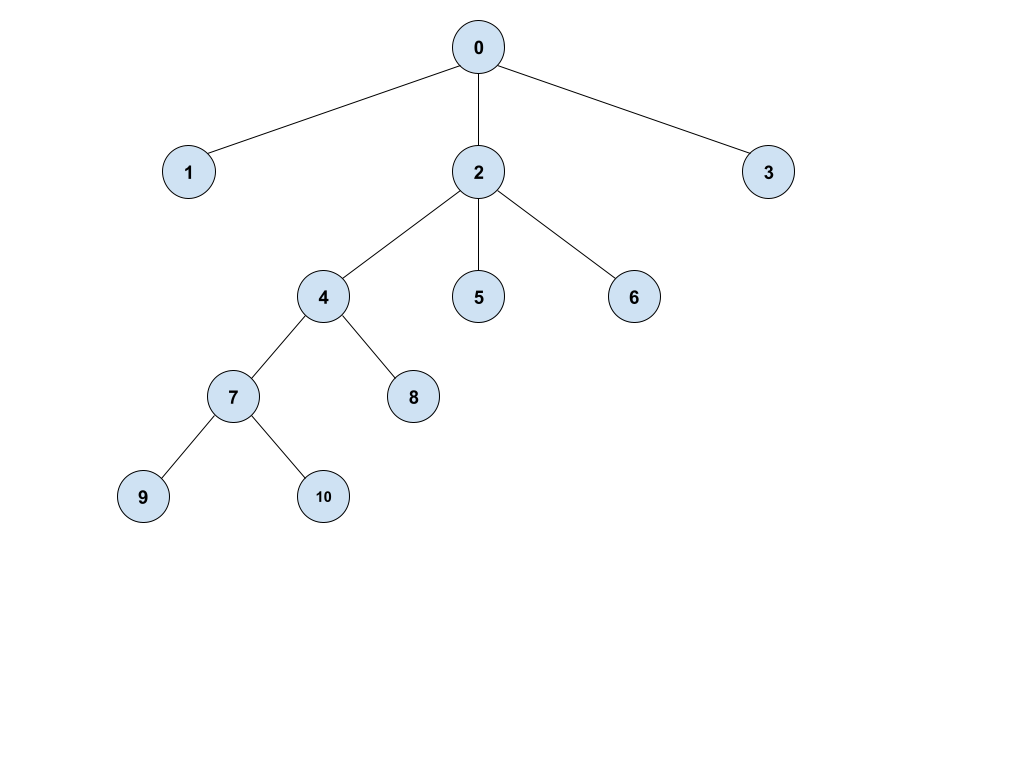
\includegraphics[width=0.9\linewidth]{images/LRMplanning.PNG}
        %     % \caption{} %% optional caption
            \label{fig:tree}
        \end{figure}

        \end{enumerate}

    \pagebreak
    %% End of Values %%%%%%%%%%%%%%%%%%%%%%%%%%%%%%%%%%%%%%%%%%%%%%%%%%%%%%



%%%%%%%%%%%%%%%%%%%%%%%%%%%%%%%%%%%%%%%%%%%%%%%%%%%%%%%%%%%%%%%%%%%%%%%%
    \subsection{Types}
    \label{sec:types}

    \pagebreak
    %% End of Values %%%%%%%%%%%%%%%%%%%%%%%%%%%%%%%%%%%%%%%%%%%%%%%%%%%%%%




%%%%%%%%%%%%%%%%%%%%%%%%%%%%%%%%%%%%%%%%%%%%%%%%%%%%%%%%%%%%%%%%%%%%%%%%
    \subsection{Definitions and Expressions}
    \label{sec:expr}

        \hspace{1cm}\begin{minipage}[h]{1\textwidth}
        \begin{grammar}
            % defn ::= Val
            <def> ::= \texttt{(}\ \texttt{val} \hyperref[subsec:id]{$ident$} $expr$ \texttt{)}\
            % defn ::= Expr
            \alt $expr$

            % expr ::= lit
            <expr> ::= $literal$
            % expr ::= var
            \alt \hyperref[subsec:id]{$ident$}
            % expr ::= unary
            \alt \hyperref[subsec:op]{\emph{unary-operator}} $expr$
            % expr ::= bin
            \alt \texttt{(}\ \hyperref[subsec:op]{\emph{binary-operator}} $expr$ $expr$ \texttt{)}
            % expr ::= Application
            \alt \texttt{(}\ \hyperref[subsec:id]{$ident$} \big\{\emph{expr}\big\} \texttt{)}
            % expr ::= let
            \alt \texttt{(}\ \texttt{let} \texttt{(}\  \texttt{[}\hyperref[subsec:id]{$ident$} $expr$\texttt{]}  \big\{\texttt{[}\hyperref[subsec:id]{$ident$} $expr$\texttt{]}\big\} \texttt{)}\ $expr$  \texttt{)}
            % expr ::= if
            \alt \texttt{(}\ \texttt{if} $expr$ $expr$ $expr$ \texttt{)}
            % expr ::= lambda
            \alt \texttt{(}\ \texttt{lambda} (\ \big\{$arguments$\big\} )\ $expr$ \texttt{)}

            <literal> ::=  \hyperref[subsec:intlit]{\emph{integer-literal}} |  \hyperref[subsec:boollit]{\emph{boolean-literal}} | \hyperref[subsec:charlit]{\emph{character}} | \hyperref[subsec:key]{leaf}

            <arguments> ::= $\epsilon$
            \alt \hyperref[subsec:id]{$ident$} :: $arguments$
            

        \end{grammar}
        \end{minipage}

        Expressions are values or parenthetical expressions.

        \subsubsection{Values}
        see \hyperref[sec:values]{Values}.


        


        \subsubsection{Parenthetical expressions} Parenthetical expressions are always withing parentheses and include function application, lambda expressions, global and local definitions, binary and unary operations, and if-statements. In the above concrete syntax, the parentheses in this font, \texttt{( ... )}, are syntax requirements, rather than denoting a grouping which is given by ( ... )

        \subsubsection{Function application}
        Function application in (g)ROOT always returns a value, and is written as the function \texttt{ID} followed by a list of zero or more expressions, which are its arguments. The arguments are not separated from the ID by parentheses. (g)ROOT has first-class functions, therefore functions can be passed as arguments. Currying is allowed.

        Example:

\cbcolor{dkgreen}
\cbstart
\begin{lstlisting}
(foo)
(bar a b)
((baz x) y)
\end{lstlisting}
\cbend

        \subsubsection{Lambda Expression}
        Lambda expressions are accomplished with the \texttt{lambda} keyword, a parentheses-enclosed list of 0 or more identifiers as formal arguments, followed by the expression that may use those arguments and/or any free variables. Nesting of lambda expressions is not allowed.

        Example:

\cbcolor{dkgreen}
\cbstart
\begin{lstlisting}
(lambda () #t)
(lambda (x) x)
(lambda (x y) (+ x y))

(lambda (a) (add2 a b))
\end{lstlisting}
\cbend

        \subsubsection{Global definitions} Global definitions are accomplished using the \texttt{val} keyword, followed by an identifier, followed by the expression which is to be bound to that value.

        Example:

\cbcolor{dkgreen}
\cbstart
\begin{lstlisting}
(val x 4)
(val y (+ x 5))
(val foo (lambda (arg) ( * arg arg)))
\end{lstlisting}
\cbend

        Calling a global definition with a preexisting identifier will re-bind that identifier to the new value - onlys allowed at the top level, and new definition must always of the same type as the previous definition.

        \subsubsection{Local definitions} Local definitions are found with the \texttt{let} expressions, which is the \texttt{let} keyword followed by the identifier(s) and the expression(s) to be bound to it, followed by the expression that local variable may be used. Let expressions must have at least one local binding. 

        Example:

\cbcolor{dkgreen}
\cbstart
\begin{lstlisting}
(let ([x 4]) (+ 2 x))    (; return 6 ;) 
(let ([x 4]) x)          (; return 4 ;) 
(let () y)               (; not allowed! ;)
\end{lstlisting}
\cbend

        Variables defined within the let binding are not defined outside of it, while variables globally relative to the let can be accessed within it. Since let bindings are a type of expression, this allows for chained let bindings.  

        Example:

\cbcolor{dkgreen}
\cbstart
\begin{lstlisting}
(let x 4 
    (let y 5 
        (let z 9 
            (+ x (- y z)))))
\end{lstlisting}
\cbend

        \subsubsection{If-expression}
        If-expressions are the only form of control flow in (g)ROOT, and are always formed with the \texttt{if} keyword followed by three expressions (the \emph{condition}, the \emph{true case} and the \emph{false case}). Omission of the false case is a syntax error, and the expressions are not separated by parentheses, brackets, or keywords.
        
        Example:

\cbcolor{dkgreen}
\cbstart
\begin{lstlisting}
(if #t 1 2)
(if (< 3 4) 
    (+ x y) 
    (- x y))
\end{lstlisting}
\cbend

        \subsubsection{Unary operators} Unary operations (used for boolean or signed negation) must not be enclosed in parentheses. They are accomplished with a unary operator in front of the expression they negate.

        Example:

\cbcolor{dkgreen}
\cbstart
\begin{lstlisting}
-3
-(+ 3 4)
-(if #t 2 3)
-x

!#t
!x
!(expr)
\end{lstlisting}
\cbend

        \subsubsection{Binary operators} The general use of binary operators is as follows: (\ \hyperref[subsec:op]{\emph{binary-operator}} $expr_1$ $expr_2$)

        The \textbf{arithmetic operators} (\ \texttt{+\ ,\ -\ ,\ *\ ,\ /\ ,\ mod }) take two expressions that evaluate to \hyperref[sec:values]{integers}. 

        The \textbf{comparator operators} (\ \texttt{==\ ,\ \textless\ ,\ \textgreater\ ,\ $\leq$ ,\ $\geq$\ ,\ != }) take two expressions that both evaluate to either \hyperref[sec:values]{integers} or \hyperref[sec:values]{booleans}.

        The \textbf{boolean operators} (\ \texttt{\&\& ,\ \textcolor{red}{||} }) take two expressions that evaluate to \hyperref[sec:values]{booleans}.





\pagebreak
%% End of Expressions %%%%%%%%%%%%%%%%%%%%%%%%%%%%%%%%%%%%%%%%%%%


    %%%%%%%%%%%%%%%%%%%%%%%%%%%%%%%%%%%%%%%%%%%%%%%%%%%%%%%%%%%%%%%%%%%%%%%%
    \subsection{Functions}
    \label{sec:func}

        \subsubsection{Built-In Functions}
        \textbf{Note}: Throughout this section, the character pair \texttt{tr} is used as shorthand to represent a tree value, an identifier bound to a tree value.

        There are four built-in functions which are integral to the tree data type. It is a checked-runtime error to call \texttt{elm, sib, cld} on a \texttt{leaf}:
        \begin{enumerate}
            \item \texttt{elm}

            Usage: \texttt{(elm tr)}

            Purpose: returns the element of the provided tree value \texttt{(tr)}

            \item \texttt{sib}

            Usage: \texttt{(sib tr)}

            Purpose: returns the sibling tree of the provided tree value \texttt{(tr)}

            \item \texttt{cld}

            Usage: \texttt{(cld tr)}

            Purpose: returns the child tree of the provided tree value \texttt{(tr)}

            \item \texttt{leaf?}
            
            Usage: \texttt{(leaf? tr)}

            Purpose: Returns boolean val \texttt{\#t} iff \texttt{tr} is a leaf.

            \item \texttt{tree}

            Usage: \texttt{(tree ELEMENT SIBLING CHILD)}

            Purpose: constructs a tree value containing the value ELEMENT, with sibling SIBLING and child CHILD
        \end{enumerate}

        \subsubsection{Standard Library Functions}
        \textbf{Note}: Throughout this section, the character pair \texttt{tr} is used as shorthand to represent a tree value, an identifier bound to a tree value.

        The first set of functions introduced in the standard library allow for programmers to use some of their beloved list functions present in other languages:
        \begin{enumerate}
            \item \texttt{(cons a b)}
            
            Creates a 1-ary tree approximating the functionality of single-dimensional list in other functional languages. \texttt{a} is any value not a tree, \texttt{b} may be \texttt{leaf} or \texttt{nil}.

            \item \texttt{(car tr)}
            
            Extracts the first value in the pair.

            \item \texttt{(cdr tr)}
            
            Extracts the second value in the pair.

            \item \texttt{(null? tr)}
            
            A predicate function that evaluates to true iff the pseudo-list is empty.

            \item \texttt{(val nil leaf)}
            
            A value \texttt{nil} that mirrors the built-in keyword leaf.

            \item \texttt{(append xs ys)}
            
            Append the list of elements in \texttt{ys} to the end of \texttt{xs}.

            \item \texttt{(revapp xs ys)}
            
            Append the list of elements in \texttt{ys} to the reverse of \texttt{xs}.

            
        \end{enumerate}

        Now some useful tree functions!
        \begin{enumerate}
            \item \texttt{(graft oak fir)}
            
            Appends a sibling tree \texttt{fir} to some other tree \texttt{oak}. The result of calling this function is a new tree in which \texttt{fir} is the rightmost sibling of \texttt{oak}. This function is extremely useful when re-shaping trees.

            \item \texttt{(level-flatten tr)} 
            
            Flattens the provided tree to a 1-ary tree, arranging elements in level-order.

            \item \texttt{(pre-flatten tr)}
            
            Flattens the provided tree to a 1-ary tree, arranging elements in pre-order.
            
            \item \texttt{(post-flatten tr)}
            
            Flattens the provided tree to a 1-ary tree, arranging elements in post-order.
            
            \item \texttt{(map f tr)}
            Maps a function \texttt{f} over every element of the provided tree \texttt{tr}.
            
            \item \texttt{(filter p? tr)}
            
            Constructs a new tree containing only elements that satisfy the predicate function \texttt{p?}, which must return a boolean value.
            
            \item \texttt{(level-fold fn base tr)}
            
            Folds a tree, visiting each element in a level-order traversal. Note that the accumulation function \texttt{fn} must take TWO arguments, the first of which is the current element, and second is the rest of the tree.
            
            \item \texttt{(pre-fold fn base tr)}
            
            Folds a tree, visiting each element in a pre-order traversal. Note that the accumulation function \texttt{fn} must take TWO arguments, the first of which is the current element, and second is the rest of the tree.

            \item \texttt{(post-fold fn base tr)}
            
            Folds a tree, visiting each element in a post-order traversal. Note that the accumulation function \texttt{fn} must take TWO arguments, the first of which is the current element, and second is the rest of the tree.
            
            \item \texttt{(fold fn base tr)}
            
            Folds a tree, in a more intuitively tree-like manner. Note that the accumulation function \texttt{fn} must take THREE arguments: the value of the current node, the sibling accumulator, and the child.accumulator.
            
            \item \texttt{(node-count tr)}
            
            Evaluates to the number of nodes in the provided tree.
            
            \item \texttt{(height tr)}
            
            Evaluates to the height of the provided tree.

        \end{enumerate}

        Higher-Order Functions:
        \begin{enumerate}
            \item \texttt{(curry f)}
            
            Allows for the partial application of a two-argument function.
            
            \item \texttt{(uncurry f)}
            
            Uncurries a previously curried function such that both of its arguments must be provided at the same time.
            
            \item \texttt{(o f g)}
            
            Given two single-argument functions, returns a single function which is the composition of \texttt{f} and \texttt{g}.
            
            \item \texttt{(flip f)}
            
            Given a two argument function, reverses the order in which the arguments are evaluated and passed to the function.
            
            \item \texttt{(flurry f)}
            
            Given a two argument function, reverses the order in which the arguments are evaluated and passed to the function, and allows for the partial application of that function. This function both flips and curries \texttt{f} (hence the fun name).

        \end{enumerate}

    \pagebreak
    %% End of Functions %%%%%%%%%%%%%%%%%%%%%%%%%%%%%%%%%%%%%%%%%%%


    %%%%%%%%%%%%%%%%%%%%%%%%%%%%%%%%%%%%%%%%%%%%%%%%%%%%%%%%%%%%%%%%%%%%%%%%
    \subsection{LRM Appendix}
    \label{sec:lrmapp}

\cbcolor{dkgreen}
\cbstart
\begin{lstlisting}
(; We can define standard list functions with our tree data type! Fun! ;)

(define (cons a b) (tree a leaf (tree b leaf leaf)))
(define (car   tr) (elm tr))
(define (cdr   tr) (cld tr))
(define (nil     ) leaf)
(define (null? tr) (leaf? tree))
   
(; a list function! ;)
(define append (xs ys)
    (if (null? xs)
        ys
        (cons (car xs) (append (cdr xs) ys))
    )
)
   
(; another list function! ;)
(define revapp (xs ys) ; (reverse xs) followed by ys
    (if (null? xs)
        ys
        (revapp (cdr xs) (cons (car xs) ys))
    )
)
   
(; appends a sibling tree (fir) to tree (oak) ;)
(define (graft oak fir)
    (if (leaf? oak)
        fir
        (tree (elm oak) (graft (sib oak) fir) (cld oak))
    )
)
   
(; attempt 4 
   this function flattens a tree, level-order ;)
(define (level-flatten tr)
    (if (leaf? tr)
        leaf
        (tree
            (elm tr)
            leaf
            (level-flatten (graft (sib tr) (cld tr)))
        )
    )
)
\end{lstlisting}
\cbend



flattening functions!

\cbcolor{dkgreen}
\cbstart
\begin{lstlisting}
(; this function flattens a tree, pre-order ;)
(define (pre-flatten tr)
    (if (leaf? tr)
        leaf
        (tree
            (elm tr)
            leaf
            (pre-flatten (graft (cld tr) (sib tr)))
        )
    )
)
   
   
(; this function flattens a tree, post-order ;)
(define (post-flatten tr)
    (if (leaf? tr)
        leaf
        (if (leaf? (cld tr))
            (tree
                (elm tr)
                leaf
                (post-flatten (sib tr)))
            (post-flatten (graft
                                (graft
                                    (cld tr)
                                    (tree (elm tr) leaf leaf))
                                (sib tr))
            )
        )
    )
)
\end{lstlisting}
\cbend


Let's create some higher order functions! Yay!

\cbcolor{dkgreen}
\cbstart
\begin{lstlisting}
(define (curry   f)   (lambda (x)   (lambda (y) (f x y))))
(define (uncurry f)   (lambda (x y) ((f x) y)))
(define (o       f g) (lambda (x)   (f (g x))))
(define (flip    f)   (lambda (x)   (lambda (y) (f y x))))


\end{lstlisting}
\cbend



function: (flurry func)
\begin{itemize}
    \item precondition:
    
    func is a function that takes exactly two args

    \item evalutation: 
    
    evaluates to a curried form of func, where:
        \begin{enumerate}
            \item the first value passed to the curried function is treated as the second argument to (func).
            \item the second value passed to the curried function is treated as the first argument to (func).
        \end{enumerate}

    \item note: flurry is a contraction of ``flip \& curry'', and we're very proud of the wordplay there.
\end{itemize}


\cbcolor{dkgreen}
\cbstart
\begin{lstlisting}
(define flurry (func)
    (curry (lambda (a b) (func b a)))
)


(; mapping function! ;)
(define (map f tr)
    (if (leaf? tr)
        leaf
        (tree
            (f (elm tr))
            (map f (sib tr))
            (map f (cld tr))
        )
    )
)
   

(; filter function! ;) 
(define filter (p? tr)
    (if (leaf? tr)
        leaf
        (if (p? (elm tr))
            (tree (elm tr) (filter p? (sib tr)) (filter p? (cld tr)))
            (filter p? (graft (cld tr) (sib tr)))
        )
    )
)
   
   
   

(; folding functions! ;) 

(; attempt 4 
   this function folds a tree, level-order ;) 
(define (level-fold fn base tr)
    (if (leaf? tr)
        base
        (fn
            (elm tr)
            (level-fold (graft (sib tr) (cld tr)))
        )
    )
)
   
(; this function folds a tree, pre-order ;) 
(define (pre-fold fn base tr)
    (if (leaf? tr)
        base
        (fn
            (elm tr)
            (pre-fold (graft (cld tr) (sib tr)))
        )
    )
)
   
(; this function folds a tree, post-order ;) 
(define (post-fold fn base tr)
    (if (leaf? tr)
        base
        (if (leaf? (cld tr))
            (fn (elm tr) (post-fold (sib tr)))
            (post-fold (graft
                            (graft (cld tr) (tree (elm tr) leaf leaf))
                                (sib tr)
                        )
            )
        )
    )
)
   
(; once we implement first-class functions, we 
   should find that the behaviors of these three
   functions are exactly equivalent to their
   lower-class cousins ;) 
(define (level-fold-flatten tr) (level-fold cons nil tr))
(define (pre-fold-flatten   tr) (pre-fold   cons nil tr))
(define (post-fold-flatten  tr) (post-fold  cons nil tr))

(; this function folds a tree, in a more intuitively 
   tree-like manner
   fn must take in three params: 
   - the current value   
   - the sibling accumulator
   - the child accumulator ;)     
(define (fold fn base tr)
    (if (leaf? tr)
        base
        (fn
            (elm tr)
            (fold fn base (sib tr))
            (fold fn base (cld tr))
        )
    )
)
   
   

(; some more fun folding functions! ;) 
(define (node-count tr)
    (pre-fold (lambda (elem count) (+ 1 count)) 0 tr)
)
   
(; this uses the tree fold to calculate the height! ;) 
(define (height tr)
    (fold
        (lambda (elem clds sibs) (+ 1 (max clds sibs)))
        0 tr
    )
)

(define (height-no-fold tr)
    (if (leaf? tr)
        0
        (max (height (sib tr)) 
            (+ 1 (height (cld tr)))
        )
    )
)
\end{lstlisting}
\cbend

    % \pagebreak
    %% End of LRM Appendix %%%%%%%%%%%%%%%%%%%%%%%%%%%%%%%%%%%%%%%%%%%

\pagebreak
%%%%%%%%%%%%%%%%%%%%%%%%%%%%%%%%%%%%%%%%%%%%%%%%%%%%%%%%%%%%%%%%%%%%%%%%%%%%%%%
%%%%%%%%%%%%%%%%%%%%%%%%%%%%%%%%%%%%%%%%%%%%%%%%%%%%%%%%%%%%%%%%%%%%%%%%%%%%%%%
%%%%%%%%%%%%%%%%%%%%%%%%%%%%%%%%%%% LRM %%%%%%%%%%%%%%%%%%%%%%%%%%%%%%%%%%%%%%%
%%%%%%%%%%%%%%%%%%%%%%%%%%%%%%%%%%%%%%%%%%%%%%%%%%%%%%%%%%%%%%%%%%%%%%%%%%%%%%%
%%%%%%%%%%%%%%%%%%%%%%%%%%%%%%%%%%%%%%%%%%%%%%%%%%%%%%%%%%%%%%%%%%%%%%%%%%%%%%%







%%%%%%%%%%%%%%%%%%%%%%%%%%%%%%%%%%%%%%%%%%%%%%%%%%%%%%%%%%%%%%%%%%%%%%%%%%%%%%%
%%%%%%%%%%%%%%%%%%%%%%%%%%%%%%%%%%%%%%%%%%%%%%%%%%%%%%%%%%%%%%%%%%%%%%%%%%%%%%%
%%%%%%%%%%%%%%%%%%%%%%%%%%%%%%%%%% PLAN %%%%%%%%%%%%%%%%%%%%%%%%%%%%%%%%%%%%%%%
%%%%%%%%%%%%%%%%%%%%%%%%%%%%%%%%%%%%%%%%%%%%%%%%%%%%%%%%%%%%%%%%%%%%%%%%%%%%%%%
%%%%%%%%%%%%%%%%%%%%%%%%%%%%%%%%%%%%%%%%%%%%%%%%%%%%%%%%%%%%%%%%%%%%%%%%%%%%%%%
\section{Project Plan}
\label{sec:PLAN}

    \subsection{Planning, Specification, and Development}

      Initial planning involved going through several different ideas for a language before we settled on a functional language with an achievable feature that stands out. Most members of the group primarily had experience with imperative languages, so this topic provided an interesting challenge for everyone. 

      We came up with a preliminary syntax for which we could parse and described in our LRM. The syntax was finalized (to include definitions) once parsing of expressions worked and as we moved on to more complex phases of the compiler. 

      We used GitLab for organization and version control, and relied on clear communication over text, Discord, and in-person to keep each other up-to-date with responsibilities, new tasks, scheduling, road blocks, and goals reached. Every feature was worked on a separate branch, and merges were usually done as a group to resolve merge conflicts between branches together, if any. 

      Phase 1 (Scanner/Parser) was done as a group. In subsequent phases, different tasks were divided amongsts group members depending on interest, with frequent collaboration with project mentor and other members as the need arises and to double-check each others work. Different responsibilities are described below.

      We did not have an official style-guide, and relied on everyone to keep their work readable and well-documented. A few final passes through each file was done to ensure good style. 

    \pagebreak




    \subsection{Project Timeline}
      For the most part, we tried to finish as much of a deliverable as possible before a given deadline. For subtasks without any hard due dates, finish-dates became more ambiguous, because a member's work tested by another member of the group, often times, revealed a new bug or a new feature that needs to be implemented before the original task is complete. Due to some of these challenges, we often found ourselves working up to a deadline or working pass an expected finish date. 

      \begin{tabular}{|l|l|}
        \hline 
        \textbf{Goal} & \textbf{Finish or Submit Date} \\
        \hline
        Final Language Idea & Feb. 2 \\ 
        Project Proposal & Feb. 4 \\
        Phase 1 test script & Feb. 23 \\ 
        Phase 1: Scanner \& Parser & Feb. 24 \\ 
        Language Reference Manual & Feb. 28 \\
        Final Language Syntax & Mar. 5 \\
        Start planning and implementing type-inferencer & Mar. 5 \\ 
        Start planning code generation & Mar. 5 \\
        Start planning closure conversion & Mar. 11 \\
        Semant for purposes of testing Conversion and Codegen & Mar. 13 \\
        Partial Semant and Codegen Module that forces a printing & Mar. 11 \\
        New phase 2 test script and reference outputs for all phases & Mar. 24 \\ 
        Phase 2: Hello World & Mar. 28 \\
        Conversion & Apr. 15 \\
        Codegen & Apr. 19 \\
        Extended Test Suite & Apr. 20 \\ 
        Type Inferencer & Apr. 23 \\ 
        Start Monomorphization to deal with infer's polymorphic types & Apr. 23 \\ 
        Debug Conversion \& Codegen & Apr. 29 \\
        thread primitives through each module & Apr. 29 \\
        Debug Infer & May 2 \\ 
        Mono & May 2 \\ 
        Create HAST \& Hof (conversion I) phase and & \\ 
        \hspace*{0.5cm}fit with Conversion (conversion II) to allow HOFs & May 5 \\
        Extend testing script & May 5 \\
        Presentation slides & May 5 \\
        Presentation & May 6 \\ 
        Final Paper \& Submission & May 7 \\ 
        \hline
      \end{tabular}

    \pagebreak




    \subsection{Roles and Responsibilities}
      These were the originally assigned recommended roles: 

      \begin{center}
      \begin{tabular}{ll}
        \hline 
        Name & Role \\ 
        \hline 
        Eliza Encherman & Manager \\ 
        Sam Russo & Tester \\
        Zachary Goldstein & Language Guru\\
        Nickolas Gravel & System Architect\\
        Amy Bui & Facilitator\\
        \hline 
      \end{tabular}
      \end{center}

      As the project progressed and implementing features of a functional language became more difficult, we abandoned these roles and each subgroup or member focused on progressively implementing different language features. Everyone was responsible intially testing their own feature and subsequent debugging, but we were also responsible for checking each others work and providing ``fresh eyes'' when testing someone else's implemented feature. Here is a list of each person's primary responsibility: 

      \begin{center}
        \begin{tabular}{ll}
          \hline 
          Name & Responsibilities \\ 
          \hline 
          Eliza Encherman & Primitive recognition and testing in Scanner/Parser, \\ 
          & Scope, Infer, Conversion, and primitive code generation \\ 
          Sam Russo & Type Inferencer  \\
          Zachary Goldstein & Errors \& Warnings, test suite, Docker environment \\
          Nickolas Gravel & Type Inferencer \\
          Amy Bui & monomorphizer, conversion I \& II, codegen\\
          \hline 
        \end{tabular}
        \end{center}



    \pagebreak




    \subsection{Development Tools}

    \pagebreak


    \pagebreak
    \subsection{Project Logs}

    \begin{figure}[h]
        \centering
        \fbox{\includegraphics[width=1\linewidth]{images/log\_dev.png}}
    \end{figure}


    \begin{figure}[h]
        \centering
        \begin{tabular}{cc}
            \begin{subfigure}{.5\textwidth}
                \centering
                \includegraphics[width=1\textwidth,height=3.8cm]{images/log\_amy.png}
                \label{fig:Amy}
            \end{subfigure} &
            \begin{subfigure}{.5\textwidth}
                \centering
                \includegraphics[width=1\textwidth,height=3.8cm]{images/log\_nik.png}
                \label{fig:Nik}
            \end{subfigure} \\ 
            \begin{subfigure}{.5\textwidth}
                \centering
                \includegraphics[width=1\textwidth,height=3.8cm]{images/log\_zach1.png}
                \label{fig:Zach}
            \end{subfigure} &
            \begin{subfigure}{.5\textwidth}
                \centering
                \includegraphics[width=1\textwidth,height=3.8cm]{images/log\_sam1.png}
                \label{fig:Zam}
            \end{subfigure} \\
            \begin{subfigure}{.5\textwidth}
                \centering
                \includegraphics[width=1\textwidth,height=3.8cm]{images/log\_eliza1.png}
                \label{fig:Eliza}
            \end{subfigure} &
        \end{tabular}
        % \label{fig:MULTI_NAME}
    \end{figure}


\pagebreak
%%%%%%%%%%%%%%%%%%%%%%%%%%%%%%%%%%%%%%%%%%%%%%%%%%%%%%%%%%%%%%%%%%%%%%%%%%%%%%%
%%%%%%%%%%%%%%%%%%%%%%%%%%%%%%%%%%%%%%%%%%%%%%%%%%%%%%%%%%%%%%%%%%%%%%%%%%%%%%%
%%%%%%%%%%%%%%%%%%%%%%%%%%%%%%%%%% PLAN %%%%%%%%%%%%%%%%%%%%%%%%%%%%%%%%%%%%%%%
%%%%%%%%%%%%%%%%%%%%%%%%%%%%%%%%%%%%%%%%%%%%%%%%%%%%%%%%%%%%%%%%%%%%%%%%%%%%%%%
%%%%%%%%%%%%%%%%%%%%%%%%%%%%%%%%%%%%%%%%%%%%%%%%%%%%%%%%%%%%%%%%%%%%%%%%%%%%%%%






%%%%%%%%%%%%%%%%%%%%%%%%%%%%%%%%%%%%%%%%%%%%%%%%%%%%%%%%%%%%%%%%%%%%%%%%%%%%%%%
%%%%%%%%%%%%%%%%%%%%%%%%%%%%%%%%%%%%%%%%%%%%%%%%%%%%%%%%%%%%%%%%%%%%%%%%%%%%%%%
%%%%%%%%%%%%%%%%%%%%%%%%%%%%%%%%% DESIGN %%%%%%%%%%%%%%%%%%%%%%%%%%%%%%%%%%%%%%
%%%%%%%%%%%%%%%%%%%%%%%%%%%%%%%%%%%%%%%%%%%%%%%%%%%%%%%%%%%%%%%%%%%%%%%%%%%%%%%
%%%%%%%%%%%%%%%%%%%%%%%%%%%%%%%%%%%%%%%%%%%%%%%%%%%%%%%%%%%%%%%%%%%%%%%%%%%%%%%
\section{Architectural Design}
\label{sec:DESIGN}

    \begin{figure}[h]
        \centering
        \fbox{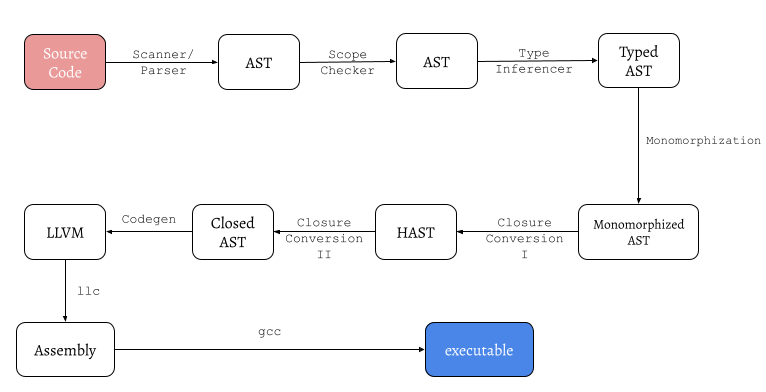
\includegraphics[width=1.1\linewidth]{images/phases.png}}
    \end{figure}
    

\pagebreak
%%%%%%%%%%%%%%%%%%%%%%%%%%%%%%%%%%%%%%%%%%%%%%%%%%%%%%%%%%%%%%%%%%%%%%%%%%%%%%%
%%%%%%%%%%%%%%%%%%%%%%%%%%%%%%%%%%%%%%%%%%%%%%%%%%%%%%%%%%%%%%%%%%%%%%%%%%%%%%%
%%%%%%%%%%%%%%%%%%%%%%%%%%%%%%%%% DESIGN %%%%%%%%%%%%%%%%%%%%%%%%%%%%%%%%%%%%%%
%%%%%%%%%%%%%%%%%%%%%%%%%%%%%%%%%%%%%%%%%%%%%%%%%%%%%%%%%%%%%%%%%%%%%%%%%%%%%%%
%%%%%%%%%%%%%%%%%%%%%%%%%%%%%%%%%%%%%%%%%%%%%%%%%%%%%%%%%%%%%%%%%%%%%%%%%%%%%%%











%%%%%%%%%%%%%%%%%%%%%%%%%%%%%%%%%%%%%%%%%%%%%%%%%%%%%%%%%%%%%%%%%%%%%%%%%%%%%%%
%%%%%%%%%%%%%%%%%%%%%%%%%%%%%%%%%%%%%%%%%%%%%%%%%%%%%%%%%%%%%%%%%%%%%%%%%%%%%%%
%%%%%%%%%%%%%%%%%%%%%%%%%%%%%%%%%% TEST %%%%%%%%%%%%%%%%%%%%%%%%%%%%%%%%%%%%%%%
%%%%%%%%%%%%%%%%%%%%%%%%%%%%%%%%%%%%%%%%%%%%%%%%%%%%%%%%%%%%%%%%%%%%%%%%%%%%%%%
%%%%%%%%%%%%%%%%%%%%%%%%%%%%%%%%%%%%%%%%%%%%%%%%%%%%%%%%%%%%%%%%%%%%%%%%%%%%%%%
\section{Test Plan}
\label{sec:TEST}

\pagebreak
%%%%%%%%%%%%%%%%%%%%%%%%%%%%%%%%%%%%%%%%%%%%%%%%%%%%%%%%%%%%%%%%%%%%%%%%%%%%%%%
%%%%%%%%%%%%%%%%%%%%%%%%%%%%%%%%%%%%%%%%%%%%%%%%%%%%%%%%%%%%%%%%%%%%%%%%%%%%%%%
%%%%%%%%%%%%%%%%%%%%%%%%%%%%%%%%%% TEST %%%%%%%%%%%%%%%%%%%%%%%%%%%%%%%%%%%%%%%
%%%%%%%%%%%%%%%%%%%%%%%%%%%%%%%%%%%%%%%%%%%%%%%%%%%%%%%%%%%%%%%%%%%%%%%%%%%%%%%
%%%%%%%%%%%%%%%%%%%%%%%%%%%%%%%%%%%%%%%%%%%%%%%%%%%%%%%%%%%%%%%%%%%%%%%%%%%%%%%





%%%%%%%%%%%%%%%%%%%%%%%%%%%%%%%%%%%%%%%%%%%%%%%%%%%%%%%%%%%%%%%%%%%%%%%%%%%%%%%
%%%%%%%%%%%%%%%%%%%%%%%%%%%%%%%%%%%%%%%%%%%%%%%%%%%%%%%%%%%%%%%%%%%%%%%%%%%%%%%
%%%%%%%%%%%%%%%%%%%%%%%%%%%%%%%% LESSON %%%%%%%%%%%%%%%%%%%%%%%%%%%%%%%%%%%%%%%
%%%%%%%%%%%%%%%%%%%%%%%%%%%%%%%%%%%%%%%%%%%%%%%%%%%%%%%%%%%%%%%%%%%%%%%%%%%%%%%
%%%%%%%%%%%%%%%%%%%%%%%%%%%%%%%%%%%%%%%%%%%%%%%%%%%%%%%%%%%%%%%%%%%%%%%%%%%%%%%
\section{Lessons Learned}
\label{sec:LESSON}

    \subsection{Amy Bui}

    My main takeaway is that compiler writing, or even writing just a single optimization for a compiler, is a very complicated endeavor. We did not end up with a lot of our original goals and features we intended for our functional language, but the detours we took while exploring this whole other paradigm was very enriching, and I was never bored and always challenged. Everyone should write a compiler at least once before graduating. This was a great project in demonstrating the practical application of the concepts and theory we learnt in 170 and 105, and I'd recommend taking both classes before 107 or at the same time for a more comfortable time. I have a lot of appreciation for people who do research and contribute to the field of functional languages, and the complexity of lambda calculus. My advice to future students is that you should have a burning desire to implement type inferencing and lambda calculus before you settle on a a functional language as your project topic; I never knew how much we took static typing and statment blocks for granted. Or you can get a thrill from just taking on this challenge. 
    
    \subsection{Nickolas Gravel}
        \begin{itemize}
            \item Takeaway: Compiler writing is a long, long journey filled with
            various pitfalls, unexpected challenges, dragons, and possibly avocados.
            For myself, I found the learning curve to be slightly steeper than my peers.
            Before this class, I had not taken CS105 Programming Languages or had
            any experience coding in a functional language. So, in the beginning, 
            I encountered some tribulation understanding these concepts. Effectively,
            I not only needed to learn the basics of compiler writing, but needed
            to learn the basic components of a programming language, and the basics
            of coding in a functional language as well.
            
            Then came type inferencing, a module that we had greatly underestimated
            the amount of time and work it would take to implement. I was one of the main
            programmers that worked on implementing this module. Again, I found
            that having some previous experience with type inferencing would have
            been a huge help here...but we persevered! I dove into the Hadley-Milner 
            type system algorithm, and with the guidance of Mert and Michael Ryan
            Clarkson, after about a month of coding the and a week of debugging
            we had a working type inferencer! 
            
            All in all, building a compiler is no joke. Even seemingly trivial
            steps in implementing a compiler were found to be not so trivial,
            requiring us to brain storm creative solutions to get to the next step. 
            For anyone building a compiler, I recommend spending ample time writing
            up a thorough design. Having a written design indicating which data
            structures and data types were being passed and returned from each
            module would have helped in overall organization and may have 
            prevented some of the various bugs that we encountered. Future students, 
            if you are set on building a language with inferred types make sure
            you have a strong understanding how to implement type inferencing and
            design your inferencer thoroughly before implementing it.
            
            Designing a programming language and building a compiler for it was
            riveting experience. I learned so much about functional languages,
            type inferencing, and what it really takes to compile source code
            down to a final executable. Everyone with any interest in low-level 
            programming should take this course, but I would recommend taking a
            course in programming languages more gradual learning curve. 


            \item Advice: 
        \end{itemize}
    
    \subsection{Sam Russo}
        \begin{itemize}
            \item Takeaway:
            \item Advice: 
        \end{itemize}
    
    \subsection{Eliza Encherman}
        \begin{itemize}
            \item Takeaway:
            \item Advice: 
        \end{itemize}
    
    \subsection{Zachary Goldstein}
        \begin{itemize}
            \item Takeaway:
            \item Advice: 
        \end{itemize}

\pagebreak
%%%%%%%%%%%%%%%%%%%%%%%%%%%%%%%%%%%%%%%%%%%%%%%%%%%%%%%%%%%%%%%%%%%%%%%%%%%%%%%
%%%%%%%%%%%%%%%%%%%%%%%%%%%%%%%%%%%%%%%%%%%%%%%%%%%%%%%%%%%%%%%%%%%%%%%%%%%%%%%
%%%%%%%%%%%%%%%%%%%%%%%%%%%%%%%%%% LESSON %%%%%%%%%%%%%%%%%%%%%%%%%%%%%%%%%%%%%
%%%%%%%%%%%%%%%%%%%%%%%%%%%%%%%%%%%%%%%%%%%%%%%%%%%%%%%%%%%%%%%%%%%%%%%%%%%%%%%
%%%%%%%%%%%%%%%%%%%%%%%%%%%%%%%%%%%%%%%%%%%%%%%%%%%%%%%%%%%%%%%%%%%%%%%%%%%%%%%







%%%%%%%%%%%%%%%%%%%%%%%%%%%%%%%%%%%%%%%%%%%%%%%%%%%%%%%%%%%%%%%%%%%%%%%%%%%%%%%
%%%%%%%%%%%%%%%%%%%%%%%%%%%%%%%%%%%%%%%%%%%%%%%%%%%%%%%%%%%%%%%%%%%%%%%%%%%%%%%
%%%%%%%%%%%%%%%%%%%%%%%%%%%%%%%%%% APPENDIX %%%%%%%%%%%%%%%%%%%%%%%%%%%%%%%%%%%
%%%%%%%%%%%%%%%%%%%%%%%%%%%%%%%%%%%%%%%%%%%%%%%%%%%%%%%%%%%%%%%%%%%%%%%%%%%%%%%
%%%%%%%%%%%%%%%%%%%%%%%%%%%%%%%%%%%%%%%%%%%%%%%%%%%%%%%%%%%%%%%%%%%%%%%%%%%%%%%
\section{Appendix}
\label{sec:APPENDIX}

    \subsection{\texttt{toplevel.ml}}
    \label{app:toplevel}
    Author(s): Sam, Eliza, Amy, Nik, Zach
\begin{lstlisting}
(* Top-level of the groot compiler: scan & parse input,
   build the AST, generate LLVM IR *)

type action =
| Ast
| Name_Check
| Tast
| Mast
| Hast
| Cast
| LLVM_IR
| Compile 


let () =
let action = ref Ast in
let set_action a () = action := a in
let speclist = [
  ("-a", Arg.Unit (set_action Ast), 		"Print the AST (default)");
  ("-n", Arg.Unit (set_action Name_Check), 	"Print the AST (name-checking)");
  ("-t", Arg.Unit (set_action Tast), 		"Print the TAST");
  ("-m", Arg.Unit (set_action Mast), 	"Print the MAST");
  ("-h", Arg.Unit (set_action Hast), 	"Print the HAST");
  ("-v", Arg.Unit (set_action Cast), 	"Print the CAST");
  ("-l", Arg.Unit (set_action LLVM_IR), 	"Print the generated LLVM IR");
  ("-c", Arg.Unit (set_action Compile),
    "Check and print the generated LLVM IR");
] in


let usage_msg = 
    "usage: ./toplevel.native [-a|-n|-t|-m|-h|-v|-l|-c] [file.gt]" in
let channel = ref stdin in
Arg.parse speclist (fun filename -> channel := open_in filename) usage_msg;
let lexbuf = Lexing.from_channel !channel in
let ast = Parser.prog Scanner.tokenize lexbuf in
match !action with
(* Default action - print the AST using ast *)
| Ast -> print_string (Ast.string_of_prog ast)
(* All other action needs to generate an SAST, store in variable sast *)
| _ ->
  let ast' = Scope.check ast in
  match !action with
  | Ast -> ()
  | Name_Check -> print_string (Ast.string_of_prog ast')
  | _ ->
    let tast = Infer.type_infer ast' in
    match !action with
    | Tast -> print_string (Tast.string_of_tprog tast)
    | _ ->
      let mast = Mono.monomorphize tast in
      match !action with
      | Mast -> print_string (Mast.string_of_mprog mast)
      | _ ->
        let hast = Hof.clean mast in 
        match !action with
        | Hast -> print_string (Hast.string_of_hprog hast)
        | _ ->
        let cast = Conversion.conversion hast in
          match !action with
          | Cast -> print_string (Cast.string_of_cprog cast)
          | LLVM_IR -> 
              print_string (Llvm.string_of_llmodule (Codegen.translate cast))
          | Compile -> 
              let the_module = Codegen.translate cast in
              Llvm_analysis.assert_valid_module the_module;
              print_string (Llvm.string_of_llmodule the_module)
          | _ -> print_string usage_msg

\end{lstlisting}
    \pagebreak

    \subsection{\texttt{ast.ml}}
    \label{app:ast}
    Author(s): Sam, Eliza, Amy, Nik, Zach
\begin{lstlisting}
(* Abstract Syntax Tree (AST) for Groot *)
(* Type of Variable Names *)
type ident = string

type expr =
  | Literal of value
  | Var     of ident
  | If      of expr * expr * expr
  | Apply   of expr * expr list
  | Let     of (ident * expr) list * expr
  | Lambda  of ident list * expr
and value =
  |Char    of char
  | Int     of int
  | Bool    of bool
  | Root    of tree
and tree =
  |Leaf
  | Branch of expr * tree * tree

type defn =
  | Val of ident * expr
  | Expr of expr

type prog = defn list


(* Pretty printing functions *)
(* toString for Ast.expr *)
let rec string_of_expr = function
  | Literal(lit) -> string_of_value lit
  | Var(v) -> v
  | If(condition, true_branch, false_branch) ->
    "(if "  ^ string_of_expr condition ^ " "
    ^ string_of_expr true_branch ^ " "
    ^ string_of_expr false_branch ^ ")"
  | Apply(f, args) ->
    "(" ^ string_of_expr f ^ " "
    ^ String.concat " " (List.map string_of_expr args) ^ ")"
  | Let(binds, body)   ->
    let string_of_binding = function
        (id, e) -> "[" ^ id ^ " " ^ (string_of_expr e) ^ "]"
    in
    "(let (" ^ String.concat " " (List.map string_of_binding binds) ^ ") "
    ^ string_of_expr body ^ ")"
  | Lambda(formals, body) ->
    "(lambda (" ^ String.concat " " formals ^ ") "
    ^ string_of_expr body ^ ")"

(* toString for Ast.value *)
and string_of_value = function
  | Char(c)     -> "'" ^ String.make 1 c ^ "'"
  | Int(i)      -> string_of_int i
  | Bool(b)     -> if b then "#t" else "#f"
  | Root(tr)    -> string_of_tree tr

(* toString for Ast.tree *)
and string_of_tree = function
  | Leaf -> "leaf"
  | Branch(ex, sib, child) ->
    (* Branch type is given by "tree" string *)
    "(tree " ^ string_of_expr ex ^ " "
    ^ string_of_tree sib ^ " "
    ^ string_of_tree child ^ ")"

(* toString for Ast.defn *)
let string_of_defn = function
  | Val(id, e) -> "(val " ^ id ^ " " ^ string_of_expr e ^ ")"
  | Expr(e)    -> string_of_expr e

(* toString for Ast.prog *)
let string_of_prog defns =
    String.concat "\n" (List.map string_of_defn defns) ^ "\n"  
\end{lstlisting}
\pagebreak


    \subsection{\texttt{scanner.mll}}
    \label{app:scanner}
    Author(s): Sam, Eliza, Amy, Nik, Zach
\begin{lstlisting}
(* Header *)
{ open Parser }

(* Regular Expressions *)
let digit = ['0'-'9']
let integer = ['-']?['0'-'9']+
let alpha = ['a'-'z']
let leaf = ("leaf"|"()")
let chrcode = digit+

(* all visible characters, excluding ()'[]\;{}| *)
let ident = ['!'-'&' '*'-':' '<'-'Z' '`'-'z' '~' '|']
            ['!'-'&' '*'-':' '<'-'Z' '^'-'z' '~' '|']*


(* ToKeNiZe *)
rule tokenize = parse
  | [' ' '\n' '\t' '\r'] { tokenize lexbuf }
  | "(;"                 { comment lexbuf }
  | '('                  { LPAREN }
  | ')'                  { RPAREN }
  | '['                  { LSQUARE }
  | ']'                  { RSQUARE }
  | "tree"               { BRANCH }
  | "leaf"               { LEAF }
  | "if"                 { IF }
  | "'"                  { apos_handler lexbuf }
  | integer as ival      { INT(int_of_string ival) }
  | "#t"                 { BOOL(true) }
  | "#f"                 { BOOL(false) }
  | "lambda"             { LAMBDA }
  | "let"                { LET }
  | "val"                { VAL }
  | ident as id          { ID(id) }
  | eof                  { EOF }
  | _                    { Diagnostic.error
                            (Diagnostic.lex_error "unrecognized character" 
                            lexbuf) }
and comment = parse
  | ";)"                 { tokenize lexbuf }
  | _                    { comment lexbuf }

(* apostrophe handler *)
and apos_handler = parse
  | '('[^''']      { tree_builder lexbuf }
  | '''            { Diagnostic.error
                    (Diagnostic.lex_error "empty character literal" lexbuf) }
  | '\\'           { escaped_char_handler lexbuf }
  | _ as c         { char_builder c lexbuf }

and tree_builder = parse
  | _ { Diagnostic.error(Diagnostic.Unimplemented "in-place tree syntax") }

and char_builder c = parse
  | '''   { CHAR(c) }
  | _ { Diagnostic.error
          (Diagnostic.lex_error ("character literal contains more " 
           ^ "than one token") lexbuf) }

and escaped_char_handler = parse
  | '\\' { char_builder '\\' lexbuf }
  | '"'  { char_builder '\"' lexbuf  }
  | '''  { char_builder '\'' lexbuf  }
  | 'n'  { char_builder '\n' lexbuf  }
  | 'r'  { char_builder '\r' lexbuf  }
  | 't'  { char_builder '\t' lexbuf  }
  | 'b'  { char_builder '\b' lexbuf  }
  | ' '  { char_builder '\ ' lexbuf  }
  | chrcode as ord
         { print_string ord; if int_of_string ord > 255
           then Diagnostic.error
                (Diagnostic.lex_error "invalid escape sequence ASCII value" 
                lexbuf)
           else char_builder (Char.chr (int_of_string ord)) lexbuf }
  | _    { Diagnostic.error
          (Diagnostic.lex_error "unrecognized escape sequence" lexbuf) }
\end{lstlisting}
    \pagebreak


    \subsection{\texttt{parser.mly}}
    \label{app:parser}
    Author(s): Sam, Eliza, Amy, Nik, Zach
\begin{lstlisting}
/* Header */
%{ open Ast %}

/* Tokens */
%token LPAREN  RPAREN
%token LSQUARE RSQUARE
%token PLUS MINUS TIMES DIVIDE MOD
%token EQ NEQ LT GT LEQ GEQ AND OR NOT
%token IF
%token <char> CHAR
%token <int>  INT
%token <bool> BOOL
%token <string> ID
%token BRANCH LEAF
%token EOF
%token LAMBDA LET VAL

/* Precedence */
%nonassoc OR
%nonassoc AND
%nonassoc LT GT
%nonassoc EQ NEQ
%nonassoc LEQ GEQ
%nonassoc PLUS MINUS
%nonassoc TIMES DIVIDE
%nonassoc NEG
%nonassoc NOT
%nonassoc BRANCH LEAF


/* Declarations */
%start prog
%type <Ast.prog> prog

%%

prog:
  | defn_list EOF                 { $1 }

defn_list:
  | /* nothing */                 { [] }
  | defn defn_list                { $1 :: $2 }

defn:
  | expr                          { Expr($1) }
  | LPAREN VAL ID expr RPAREN     { Val($3, $4) }

formals_opt:
  | /* nothing */                 { [] }
  | formal_list                   { $1 }

formal_list:
  | ID                            { [$1] }
  | ID formal_list                { $1 :: $2 }


/* Rules */
value:
  | CHAR                          { Char($1) }
  | INT                           { Int($1) }
  | BOOL                          { Bool($1) }
  | tree                          { Root($1) }
  /* ! Note: tree is not a token - no need for a ROOT token while scanning */


tree:
  | LEAF                                  { Leaf }
  | LPAREN BRANCH expr tree tree RPAREN   { Branch($3, $4, $5) }


let_binding_list:
  | /* nothing */                             { [] }
  | LSQUARE RSQUARE let_binding_list  
    { Diagnostic.warning (Diagnostic.parse_warning "empty let binding" 1); $3 } 
    /* NON FATAL */
  | LSQUARE expr RSQUARE let_binding_list     
    { Diagnostic.error (Diagnostic.parse_error ("let binding must contain" 
      ^ " id and value") 2) } /* FATAL */
  | LSQUARE ID expr RSQUARE let_binding_list  { ($2, $3) :: $5 }


expr_list:
  | /* null */         { [] }
  | expr expr_list     { $1 :: $2 }


expr:
  | value                                                 { Literal($1) }
  | ID                                                    { Var($1) }
  | LPAREN expr expr_list RPAREN                          { Apply($2, $3) }
  | LPAREN LET LPAREN let_binding_list RPAREN expr RPAREN { Let($4, $6)}
  | LPAREN IF expr expr expr RPAREN                       { If($3, $4, $5) }
  | LPAREN LAMBDA LPAREN formals_opt RPAREN expr RPAREN   { Lambda($4, $6) }
\end{lstlisting}
    \pagebreak


    \subsection{\texttt{scope.ml}}
    \label{app:scope}
    Author(s): Amy, Eliza
\begin{lstlisting}
(* Name (scope) checks variable names *)
open Ast

(* toplevel naming environment, preloaded with built-ins *)
let nameEnv = List.fold_right List.cons [ "printi"; "printb"; "printc";
                                            "+"; "-"; "*"; "/"; "mod";
                                            "<"; ">"; ">="; "<="; "~";
                                            "!=i"; "=i"; "&&"; "||"; "not"  ] []

(* Takes and AST and checks if variables are bound in scope.
    Returns same AST if so, otherwise raises Unbound variable error
    if a variable is unbound. *)
let check defns =

  (* Recursively checks the scope of variables names used in an expression *)
  let rec checkExpr expression rho =
    let rec exp e = match e with
        Literal _ -> ()
      | Var id -> 
          if List.mem id rho then ()
          else Diagnostic.error (Diagnostic.Unbound id)
      | If (e1, e2, e3) ->
          let (_, _, _) = (exp e1, exp e2, exp e3) in ()
      | Apply (f, args) ->
          let _ = exp f in List.iter exp args
      | Let (bs, body) ->
          let (xs, es) = List.split bs in
          let () = List.iter exp es in
          checkExpr body (List.fold_right List.cons xs rho)
      | Lambda (formals, body) ->
          checkExpr body (List.fold_right List.cons formals rho)
    in exp expression
  in

  let rec checkDef ds env =
    match ds with
      [] -> env
    | f :: rest ->
      let env' =
        (match f with
            Val (id, exp) ->
            let () = checkExpr exp env in
            id :: env
          | Expr exp -> let () = checkExpr exp env in env)
      in checkDef rest env'
  in
  let _ = checkDef defns nameEnv in

  (* Returns the AST if no error raised *)
  defns
\end{lstlisting}
    \pagebreak



    \subsection{\texttt{tast.ml}}
    \label{app:tast}
    Author(s): Sam, Nik
\begin{lstlisting}
(* TAST -- Type inference. *)

open Ast

exception Type_error of string
let type_error msg = raise (Type_error msg)

type gtype =
  | TYCON of tycon
  | TYVAR of tyvar
  | CONAPP of conapp
and tycon =
  | TyInt
  | TyBool
  | TyChar
  | TArrow of gtype
and tyvar =
  | TVariable of int
and conapp = (tycon * gtype list)

type tyscheme = tyvar list * gtype

let inttype = TYCON TyInt
let chartype = TYCON TyChar
let booltype = TYCON TyBool
let functiontype resultType formalsTypes =
      CONAPP (TArrow resultType, formalsTypes)


(* TAST expression *)
type texpr = gtype * tx
and tx =
  | TLiteral     of tvalue
  | TypedVar     of ident
  | TypedIf      of texpr * texpr * texpr
  | TypedApply   of texpr * texpr list
  | TypedLet     of (ident * texpr) list * texpr
  | TypedLambda  of (gtype * ident) list * texpr
and tvalue = TChar of char | TInt of int | TBool of bool | TRoot of ttree
and ttree = TLeaf | TBranch of tvalue * ttree * ttree

type tdefn = TVal of ident * texpr | TExpr of texpr
type tprog = tdefn list

(* Pretty printer *)

(* String of gtypes *)
let rec string_of_ttype = function
  | TYCON ty -> string_of_tycon ty
  | TYVAR tp -> string_of_tyvar tp
  | CONAPP con -> string_of_conapp con
and string_of_tycon = function
  | TyInt -> "int"
  | TyBool -> "bool"
  | TyChar -> "char"
  | TArrow (retty) -> string_of_ttype retty
and string_of_tyvar = function
  | TVariable n -> "'" ^ string_of_int n
and string_of_conapp (tyc, tys) =
string_of_tycon tyc ^ " (" 
    ^ String.concat " " (List.map string_of_ttype tys) ^ ")"

and string_of_subs = function
  | [] -> ""
  | (t1, t2) :: cs ->
      "(" ^ string_of_tyvar t1 ^ ", " ^ string_of_ttype t2 ^ ") "
      ^ string_of_subs cs

and string_of_context = function
  | [] -> ""
  | (ident, (tvs, gt)) :: ctx ->
      "\n=: " ^ ident ^ ", (["
      ^ String.concat ", " (List.map string_of_tyvar tvs)
      ^ "], " ^ string_of_ttype gt ^ ")" ^ string_of_context ctx

and string_of_tyformals (gt, ident) =
    "(" ^ ident ^ " : " ^ string_of_ttype gt ^ ")"

(* String of a typed expression (texpr) == (type, t-expression) *)
let rec string_of_texpr (typ, exp) =
    "[" ^ string_of_ttype typ ^ "] " ^ string_of_tx exp
and string_of_tx = function
    TLiteral v -> string_of_tvalue v
  | TypedVar id -> id
  | TypedIf (te1, te2, te3) ->
    "(if "  ^ string_of_texpr te1 ^ " "
    ^ string_of_texpr te2 ^ " "
    ^ string_of_texpr te3 ^ ")"
  | TypedApply (f, args) ->
    "(" ^ string_of_texpr f ^ " "
    ^ String.concat " " (List.map string_of_texpr args) ^ ")"
  | TypedLet (binds, body) ->
    let string_of_binding (id, e) =
      "[" ^ id ^ " " ^ (string_of_texpr e) ^ "]"
    in
    "(let ("  ^ String.concat " " (List.map string_of_binding binds) ^ ") "
    ^ string_of_texpr body ^ ")"
  | TypedLambda (formals, body) ->
    let formalStringlist = List.map (fun (ty, x) ->
        string_of_ttype ty ^ " " ^ x) formals in
    "(lambda (" ^ String.concat ", "  formalStringlist
    ^ ") " ^ string_of_texpr body ^ ")"

(* toString for Sast.svalue *)
and string_of_tvalue = function
  | TChar c -> String.make 1 c
  | TInt i -> string_of_int i
  | TBool b -> if b then "#t" else "#f"
  | TRoot tr -> string_of_ttree tr

(* toString for Sast.stree *)
and string_of_ttree = function
    TLeaf -> "leaf"
  | TBranch (v, sib, child) ->
    "(tree " ^ string_of_tvalue v ^ " "
    ^ string_of_ttree sib ^ " "
    ^ string_of_ttree child ^ ")"


(* String of a typed defn (tdefn) *)
let string_of_tdefn = function
  | TVal (id, te) -> "(val " ^ id ^ " " ^ string_of_texpr te ^ ")"
  | TExpr te    -> string_of_texpr te


(* String of the tprog == tdefn list *)
let string_of_tprog tdefns =
String.concat "\n" (List.map string_of_tdefn tdefns) ^ "\n"
\end{lstlisting}
    \pagebreak


    \subsection{\texttt{infer.ml}}
    \label{app:infer}
    Author(s): Sam, Eliza, Nik
\begin{lstlisting}
open Ast
open Tast
module StringMap = Map.Make (String)

(* prims - initializes context with built-in functions with their types *)
(* prims : (id * tyvar) list * (tycon * gtype list) *)
let prims =
  [
    ("printb",  ([ TVariable (-1) ], Tast.functiontype inttype [ booltype ]));
    ("printi",  ([ TVariable (-2) ], Tast.functiontype inttype [ inttype ]));
    ("printc",  ([ TVariable (-3) ], Tast.functiontype inttype [ chartype ]));
    ("+",       ([ TVariable (-4) ], Tast.functiontype inttype [ inttype; inttype ]));
    ("-",       ([ TVariable (-4) ], Tast.functiontype inttype [ inttype; inttype ]));
    ("/",       ([ TVariable (-4) ], Tast.functiontype inttype [ inttype; inttype ]));
    ("*",       ([ TVariable (-4) ], Tast.functiontype inttype [ inttype; inttype ]));
    ("mod",     ([ TVariable (-4) ], Tast.functiontype inttype [ inttype; inttype ]));
    ("<",       ([ TVariable (-5) ], Tast.functiontype booltype [ inttype; inttype ]));
    (">",       ([ TVariable (-5) ], Tast.functiontype booltype [ inttype; inttype ]));
    ("<=",      ([ TVariable (-5) ], Tast.functiontype booltype [ inttype; inttype ]));
    (">=",      ([ TVariable (-5) ], Tast.functiontype booltype [ inttype; inttype ]));
    ("=i",      ([ TVariable (-5) ], Tast.functiontype booltype [ inttype; inttype ]));
    ( "!=i",    ([ TVariable (-5) ], Tast.functiontype booltype [ inttype; inttype ]) );
    ( "&&",     ([ TVariable (-6) ], Tast.functiontype booltype [ booltype; booltype ]) );
    ( "||",     ([ TVariable (-6) ], Tast.functiontype booltype [ booltype; booltype ]) );
    ("not",     ([ TVariable (-7) ], Tast.functiontype booltype [ booltype ]));
    ("~",       ([TVariable (-2)], Tast.functiontype inttype [inttype]))
  ]

(* is_ftv - returns true if 'gt' is equal to free type variable 'var'
    (i.e. 'gt' is a type variable and 'var' is a free type variable). For the
    conapp case, we recurse over the conapp's gtype list searching for any free
    type variables. When this function returns true it means the type variable
    is matching *)
let rec is_ftv (var : tyvar) (gt : gtype) =
  match gt with
  | TYCON _ -> false
  | TYVAR v -> v = var
  | CONAPP (_, gtlst) ->
    (* if any x in gtlst is ftv this returns true, else returns false *)
    List.fold_left (fun acc x -> is_ftv var x || acc) false gtlst

(* ftvs - returns a list of free type variables amongst a collection 
   of gtypes *)
(* retty : tyvar list *)
let rec ftvs (ty : gtype) =
  match ty with
  | TYVAR t -> [ t ]
  | TYCON _ -> []
  | CONAPP (_, gtlst) -> List.fold_left (fun acc x -> acc @ ftvs x) [] gtlst

(* fresh - returns a fresh gtype variable (integer) *)
let fresh =
  let k = ref 0 in
  (* fun () -> incr k; TVariable !k *)
  fun () -> incr k; TYVAR (TVariable !k)


(* sub - updates a list of constraints with substitutions in theta *)
let sub (theta : (tyvar * gtype) list) (cns : (gtype * gtype) list) =
  (* sub_one - takes in single constraint and updates it with substitution in theta *)
  let sub_one (cn : gtype * gtype) =
    List.fold_left
      (fun ((c1, c2) : gtype * gtype) ((tv, gt) : tyvar * gtype) ->
          match (c1, c2) with
          | TYVAR t1, TYVAR t2 ->
            if tv = t1 then (gt, c2) else if tv = t2 then (c1, gt) else (c1, c2)
          | TYVAR t1, _ -> if tv = t1 then (gt, c2) else (c1, c2)
          | _, TYVAR t2 -> if tv = t2 then (c1, gt) else (c1, c2)
          | _, _ -> (c1, c2))
      cn theta
  in
  List.map sub_one cns

(* compose - applies the substitutions in theta1 to theta2 *)
let compose theta1 theta2 =
  (* sub_one - takes a single substitution in theta1 and applies it to theta2 *)
  let sub_one cn =
    List.fold_left
      (fun (acc : tyvar * gtype) (one_sub : tyvar * gtype) ->
          match (acc, one_sub) with
          | (a1, TYVAR a2), (s1, TYVAR s2) ->
            if s1 = a1 then (s1, TYVAR a2)
            else if s1 = a2 then (a1, TYVAR s2)
            else acc
          | (a1, a2), (s1, TYVAR _) -> if a1 = s1 then (s1, a2) else acc
          | (a1, _), (s1, s2) -> if a1 = s1 then (s1, s2) else acc)
      cn theta1
  in
  List.map sub_one theta2

(* solve': solves a single constraint 'c' *)
let rec solve' (c : gtype * gtype) =
  match c with
  | TYVAR t1, TYVAR t2 -> [ (t1, TYVAR t2) ]
  | TYVAR t1, TYCON t2 -> [ (t1, TYCON t2) ]
  | TYVAR t1, CONAPP t2 ->
    if is_ftv t1 (CONAPP t2) then
      Diagnostic.error (Diagnostic.TypeError "type variable is not free type in type constructor")
    else [ (t1, CONAPP t2) ]
  | TYCON t1, TYVAR t2 -> solve' (TYVAR t2, TYCON t1)
  | TYCON (TArrow (TYVAR t1)), TYCON t2 -> [ (t1, TYCON t2) ]
  | TYCON t1, TYCON (TArrow (TYVAR t2)) -> [ (t2, TYCON t1) ]
  | TYCON t1, TYCON t2 ->
    if t1 = t2 then []
    else
      Diagnostic.error (Diagnostic.TypeError
        ("type constructor mismatch " ^ string_of_tycon t1
          ^ " != " ^ string_of_tycon t2))
  | TYCON t1, CONAPP t2 ->
    Diagnostic.error (Diagnostic.TypeError
      ("type constructor mismatch " ^ string_of_tycon t1
      ^ " != " ^ string_of_conapp t2))
  | CONAPP t1, TYVAR t2 -> solve' (TYVAR t2, CONAPP t1)
  | CONAPP t1, TYCON t2 ->
    Diagnostic.error (Diagnostic.TypeError
      ("type constructor mismatch " ^ string_of_conapp t1
        ^ " != " ^ string_of_tycon t2))
  | CONAPP t1, CONAPP t2 -> (
      match (t1, t2) with
      | (TArrow t1, tys1), (TArrow t2, tys2) ->
        solve ((t1, t2) :: List.combine tys1 tys2)
      | _ ->
        Diagnostic.error (Diagnostic.TypeError
          ("type constructor mismatch " ^ string_of_conapp t1
            ^ " != " ^ string_of_conapp t2)))


(* solve - solves a list of constraints, calls 'solver' to iterate through the
            constraint list, once constraint list has been iterated 'compose' is
            called to tie 'theta1' and 'theta2' together, returns theta *)
and solve (constraints : (gtype * gtype) list) =
  let solver cns =
    match cns with
    | [] -> []
    | cn :: cns ->
      let theta1 = solve' cn in
      let theta2 = solve (sub theta1 cns) in
      (compose theta2 theta1) @ theta2
  in solver constraints


(* generate_constraints gctx e:
      infers the type of expression 'e' and a generates a set of constraints,
      'gctx' refers to the global context 'e' can refer to.

    Type References:
        ctx : (ident * tyscheme) list == (ident * (tyvar list * gtype)) list
    tyscheme : (tyvar list * gtype)
      retty : gtype * (gtype * gtype) list * (gtype * tx) *)
let rec generate_constraints gctx e =
  let rec constrain ctx e =
    match e with
    | Literal e -> value e
    | Var name ->
      let _, (_, tau) = List.find (fun x -> fst x = name) ctx in
      (tau, [], (tau, TypedVar name))
    | If (e1, e2, e3) ->
      let t1, c1, tex1 = generate_constraints gctx e1 in
      let t2, c2, tex2 = generate_constraints gctx e2 in
      let t3, c3, tex3 = generate_constraints gctx e3 in
      let c = [ (booltype, t1); (t3, t2) ] @ c1 @ c2 @ c3 in
      let tex = TypedIf (tex1, tex2, tex3) in
      (t3, c, (t3, tex))
    | Apply (f, args) ->
      let t1, c1, tex1 = generate_constraints ctx f in
      let ts2, c2, texs2 =
        List.fold_left
          (fun acc e ->
              let t, c, x = generate_constraints ctx e in
              let ts, cs, xs = acc in
              (t :: ts, c @ cs, x :: xs))
          ([], c1, []) (List.rev args)
      in
      (* reverse args to maintain arg order *)
      let retType = fresh () in
      ( retType,
        (t1, Tast.functiontype retType ts2) :: c2,
        (retType, TypedApply (tex1, texs2)) )
    | Let (bindings, expr) ->
      let l = List.map (fun (_, e) -> generate_constraints ctx e) bindings in
      let cns = List.concat (List.map (fun (_, c, _) -> c) l) in
      let taus = List.map (fun (t, _, _) -> t) l in
      let asts = List.map (fun (_, _, a) -> a) l in
      let names = List.map fst bindings in
      let ctx_addition =
        List.map (fun (n, t) -> (n, ([], t))) (List.combine names taus)
      in
      let new_ctx = ctx_addition @ ctx in
      let b_tau, b_cns, b_tast = generate_constraints new_ctx expr in
      (b_tau, b_cns @ cns, (b_tau, TypedLet (List.combine names asts, b_tast)))
    | Lambda (formals, body) ->
      let binding = List.map (fun x -> (x, ([], fresh ()))) formals in
      let new_context = binding @ ctx in
      let t, c, tex = generate_constraints new_context body in
      let _, tyschms = List.split binding in
      let _, formaltys = List.split tyschms in
      let typedFormals = List.combine formaltys formals in
      ( Tast.functiontype t formaltys,
        c,
        (Tast.functiontype t formaltys, TypedLambda (typedFormals, tex)) )
  and value v =
    match v with
    | Int  e -> (inttype, [],  (inttype,  TLiteral (TInt e)))
    | Char e -> (chartype, [], (chartype, TLiteral (TChar e)))
    | Bool e -> (booltype, [], (booltype, TLiteral (TBool e)))
    | Root t -> tree t
  and tree t =
    match t with
    | Leaf     -> Diagnostic.error (Diagnostic.Unimplemented "contraint generation for Leaf")
    | Branch _ -> Diagnostic.error (Diagnostic.Unimplemented "contraint generation for Branch")
  in
  constrain gctx e


(* gimme_tycon_gtype - sort of a hack function that we made to solve the bug we
    came across in applying substitutions, called in tysubst *)
let gimme_tycon_gtype _ = function
  | TYCON x -> x
  | TYVAR x ->
    Diagnostic.error (Diagnostic.TypeError ("the variable " ^ string_of_tyvar x
                        ^ " has type tyvar but an expression was exprected of type tycon"))
  | CONAPP x ->
    Diagnostic.error (Diagnostic.TypeError ("the constructor " ^ string_of_conapp x
                        ^ " has type conapp but an expression was exprected of type tycon"))



(* tysubst - subs in the type in place of type variable  *)
let rec tysubst (one_sub : tyvar * gtype) (t : gtype) =
  match (one_sub, t) with
  | (x, y), TYVAR z -> if x = z then y else TYVAR z
  | _, TYCON (TArrow retty) -> TYCON (TArrow (tysubst one_sub retty))
  | _, TYCON c -> TYCON c
  | (x, _), CONAPP (a, bs) ->
    let tycn = gimme_tycon_gtype x in
    CONAPP (tycn (tysubst one_sub (TYCON a)), (List.map (tysubst one_sub)) bs)

(* get_constraints - returns a list of Tasts
        Tast : [ (ident * (gtype * tx)) ] = [ (ident * texpr) | texpr ] = [ tdefns ]
    tyscheme : (tyvar list * gtype) *)
let get_constraints (ctx : (ident * tyscheme) list) (d : defn) =
  match d with
  | Val (name, e) ->
    let t, c, tex = generate_constraints ctx e in
    (t, c, TVal (name, tex))
  | Expr e ->
    let (t, c, tex) = generate_constraints ctx e in
    (t, c, TExpr tex)


(*  input: (tyvar * gtype) list *)
(*  retty: tdefn -> tdefn *)
let apply_subs (sub : (tyvar * gtype) list) =
  match sub with
  | [] -> (fun x -> x)
  | xs ->
    let final_ans =
      (fun tdef ->
          (* xs - the list of substitutions we want to apply *)
          (* tdef - the tdefn we want to apply the substitutions to *)
          let rec expr_only_case (x : texpr) =
            List.fold_left
              (* anon fun - takes one texpr and takes one substitution and subs substitution into the texpr *)
              (fun (tast_gt, tast_tx) (tv, gt) ->
                (* updated_tast_tx - matches texpr with tx and recurses on expressions *)
                let updated_tast_tx = match tast_tx with
                  | TypedIf (x, y, z) ->
                    TypedIf (expr_only_case x, expr_only_case y, expr_only_case z)
                  | TypedApply (x, xs) ->
                    let txs = List.map expr_only_case xs in
                    TypedApply (expr_only_case x, txs)
                  | TypedLet ((its), x) -> TypedLet (List.map (fun (x, y) ->
                      (x, expr_only_case y)) its, expr_only_case x)
                  | TypedLambda (tyformals, body) ->
                    TypedLambda ((List.map (fun (x, y) -> (tysubst (tv, gt) x, y))
                                    tyformals), expr_only_case body)
                  | TLiteral x -> TLiteral x
                  | TypedVar x -> TypedVar x
                in
                let temp = (tysubst (tv, gt) tast_gt, updated_tast_tx) in temp) x xs in
          match tdef with
          | TVal (name, x) -> TVal (name, (expr_only_case x))
          (* Do we need to do anything with updating context here? *)
          | TExpr x -> TExpr (expr_only_case x)
      )
    in final_ans

(* update_ctx - if the typed definition is a TVal this function will make sure
    there are no unbound type variables and tha *)
let update_ctx ctx tydefn =
  match tydefn with
  | TVal (name, (gt, _)) ->
    (name, (List.filter (fun x -> List.exists (fun y -> y = x) (ftvs gt)) (ftvs gt), gt))::ctx
  | TExpr _ -> ctx


(* type_infer
      input : ( ident | ident * expr ) list
    returns : ( ident * (gtype * tx) ) list *)

let type_infer (ds : defn list) =
  let rec infer_defns ctx defn =
    match defn with
    | [] -> []
    | d :: ds ->
      (* get the constraints for the defn *)
      let _, cs, tex = get_constraints ctx d in
      (* subs -> (Infer.tyvar * Infer.gtype) list *)
      let subs = solve cs in
      (* apply subs to tdefns *)
      let tdefn = (apply_subs subs) tex in
      (* update ctx *)
      let ctx' = update_ctx ctx tdefn in
      (* recurse *)
      tdefn :: infer_defns ctx' ds
  in
  infer_defns prims ds

(* type_infer
      input : ( ident | ident * expr ) list
    returns : ( ident * (gtype * tx) ) list *)
\end{lstlisting}
    \pagebreak


    \subsection{\texttt{mast.ml}}
    \label{app:mast}
    Author(s): Amy
\begin{lstlisting}
(* MAST -- monomorphized AST where pholymorphism is removed *)
module StringMap = Map.Make(String)
type mname = string

type mtype =
    Mtycon of mtycon
  | Mtyvar of int
  | Mconapp of mconapp
and mtycon =
    MIntty
  | MCharty
  | MBoolty
  | MTarrow of mtype
and mconapp = (mtycon * mtype list)

let integerTy  = Mtycon MIntty
let characterTy = Mtycon MCharty
let booleanTy = Mtycon MBoolty
let functionTy (ret, args) = Mconapp (MTarrow ret, args)



type mexpr = mtype * mx
and mx =
  | MLiteral  of mvalue
  | MVar      of mname
  | MIf       of mexpr * mexpr * mexpr
  | MApply    of mexpr * mexpr list
  | MLet      of (mname * mexpr) list * mexpr
  | MLambda   of (mtype * mname) list * mexpr
and mvalue =
  | MChar     of char
  | MInt      of int
  | MBool     of bool
  | MRoot     of mtree
and mtree =
  | MLeaf
  | MBranch   of mvalue * mtree * mtree

type mdefn =
  | MVal      of mname * mexpr
  | MExpr     of mexpr


type polyty_env = mexpr StringMap.t

type mprog = mdefn list


(* Pretty printer *)
(* String of mtypes *)
let rec string_of_mtype = function
  | Mtycon ty -> string_of_mtycon ty
  | Mconapp con -> string_of_mconapp con
  | Mtyvar i -> "'" ^ string_of_int i
and string_of_mtycon = function
  | MIntty -> "int"
  | MBoolty -> "bool"
  | MCharty -> "char"
  | MTarrow (retty) -> string_of_mtype retty
and string_of_mconapp (tyc, tys) =
  string_of_mtycon tyc ^ " (" 
  ^ String.concat " " (List.map string_of_mtype tys) ^ ")"


(* String of a typed expression (mexpr) == (type, m-expression) *)
let rec string_of_mexpr (typ, exp) =
  "[" ^ string_of_mtype typ ^ "] " ^ string_of_mx exp
and string_of_mx = function
  | MLiteral v -> string_of_mvalue v
  | MVar id -> id
  | MIf (e1, e2, e3) ->
    "(if "  ^ string_of_mexpr e1 ^ " "
    ^ string_of_mexpr e2 ^ " "
    ^ string_of_mexpr e3 ^ ")"
  | MApply (f, args) ->
    "(" ^ string_of_mexpr f ^ " "
    ^ String.concat " " (List.map string_of_mexpr args) ^ ")"
  | MLet (binds, body) ->
    let string_of_binding (id, e) =
      "[" ^ id ^ " " ^ (string_of_mexpr e) ^ "]"
    in
    "(let ("  ^ String.concat " " (List.map string_of_binding binds) ^ ") "
    ^ string_of_mexpr body ^ ")"
  | MLambda (formals, body) ->
    let formalStringlist = List.map (fun (ty, x) -> string_of_mtype ty ^ " " ^ x) formals in
    "(lambda (" ^ String.concat ", "  formalStringlist
    ^ ") " ^ string_of_mexpr body ^ ")"
(* toString for Mast.mvalue *)
and string_of_mvalue = function
  | MChar c -> String.make 1 c
  | MInt i -> string_of_int i
  | MBool b -> if b then "#t" else "#f"
  | MRoot tr -> string_of_mtree tr
(* toString for Mast.mtree *)
and string_of_mtree = function
  | MLeaf -> "leaf"
  | MBranch (v, sib, child) ->
    "(tree " ^ string_of_mvalue v ^ " "
    ^ string_of_mtree sib ^ " "
    ^ string_of_mtree child ^ ")"



(* String of a mono typed defn (mdefn) *)
let string_of_mdefn = function
  | MVal (id, me) -> "(val " ^ id ^ " " ^ string_of_mexpr me ^ ")"
  | MExpr me    -> string_of_mexpr me


(* String of the mprog == mdefn list *)
let string_of_mprog mdefns =
  String.concat "\n" (List.map string_of_mdefn mdefns) ^ "\n"
\end{lstlisting}
    \pagebreak




    \subsection{\texttt{mono.ml}}
    \label{app:mono}
    Author(s): Amy
\begin{lstlisting}
(* Monopmorphizes a typed (incl poly) program *)

open Tast
open Mast


(* Function takes a tprog (list of typed definitions),
    and monomorphizes it. to produce a mprog *)
let monomorphize (tdefns : tprog) =

  (* Takes a Tast.gtype and returns the equivalent Mast.mtype *)
  let rec ofGtype = function
      TYCON ty    -> Mtycon  (ofTycon ty)
    | TYVAR tp    -> Mtyvar   (ofTyvar tp)
    | CONAPP con  -> Mconapp (ofConapp con)
  and ofTycon = function
      TyInt        -> MIntty
    | TyBool       -> MBoolty
    | TyChar       -> MCharty
    | TArrow rety  -> MTarrow (ofGtype rety)
  and ofTyvar = function
      TVariable n -> n
  and ofConapp (tyc, tys) = (ofTycon tyc, List.map ofGtype tys)
  in




  (* Takes an mtype, and returns true if it is polymorphic, false o.w. *)
  let rec isPolymorphic (typ : mtype) = match typ with
    | Mtycon  t -> poly_tycon t
    | Mtyvar  _ -> true
    | Mconapp c -> poly_conapp c
  and poly_tycon = function
      MIntty | MBoolty | MCharty -> false
    | MTarrow t -> isPolymorphic t
  and poly_conapp (tyc, mtys) =
    (poly_tycon tyc)
    || (List.fold_left (fun init mtyp -> init || (isPolymorphic mtyp))
          false mtys)
  in



  (* Takes a type environment and a string key "id". Returns the
        value (mtype) that the key mapts to. *)
  let lookup (id : mname) (gamma : polyty_env) =
    StringMap.find id gamma
  in


  (* Takes a name and an polyty_env, and inserts it into the map *)
  let set_aside (id : mname) ((ty, exp) : mexpr) (gamma : polyty_env) =
    StringMap.add id (ty, exp) gamma
  in


  (* Returns true if ty is a type variable *)
  let isTyvar (ty : mtype) = match ty with
      Mtycon _  -> false
    | Mtyvar _  -> true
    | Mconapp _ -> false
  in

  (* Returns true if ty is a function type *)
  let isFunctionType (ty : mtype) = match ty with
      Mconapp (MTarrow _, _)  -> true
    | _                       -> false
  in


  (* (fty, exp) == poly lambda expression
      (ty) == mono function type *)
  let resolve (prog : mprog) (id : mname) (ty : mtype) ((fty, exp) : mexpr) =
    (* Given a function type, returns the list of the types of the arguments *)
    let get_type_of_args = function
        Mconapp (MTarrow _, formaltys) -> formaltys
      | _ -> Diagnostic.error 
              (Diagnostic.MonoError "cannot monomorphize non-function type")
    in

    let formaltys     = get_type_of_args ty  in (* mono *)
    let polyargtys    = get_type_of_args fty in (* poly *)
    let substitutions = List.combine polyargtys formaltys in

    (* Given a (polymorphic) mtype, returns the monomorphic version *)
    let resolve_mty (mty : mtype) =
      let apply_subs typ (arg, sub) =
        if isTyvar arg
          then
            let tyvarID =
              (match arg with
                  Mtyvar i -> i
                | _ -> Diagnostic.error 
                        (Diagnostic.MonoError "non-tyvar substitution"))
            in
            let rec search_mtype = function
                Mtycon tyc -> Mtycon (search_tycon tyc)
              | Mtyvar i   -> if i = tyvarID then sub else Mtyvar i
              | Mconapp con -> Mconapp (search_con con)
            and search_tycon = function
                MIntty  -> MIntty
              | MCharty -> MCharty
              | MBoolty -> MBoolty
              | MTarrow retty -> MTarrow (search_mtype retty)
            and search_con (tyc, mtys) =
              (search_tycon tyc, List.map search_mtype mtys)
            in search_mtype typ
        else typ
      in List.fold_left apply_subs mty substitutions
    in

    (* Given an (polymorphic) mx, returns the monomorphic version, with an
        updated program, if any. *)
    let rec resolve_mx pro = function
        MLiteral l -> (MLiteral l, pro)
      | MVar     v -> (MVar v, pro)
      | MIf ((t1, e1), (t2, e2), (t3, e3)) ->
          let t1' = resolve_mty t1 in
          let t2' = resolve_mty t2 in
          let t3' = resolve_mty t3 in
          let (e1', pro1) = resolve_mx pro  e1 in
          let (e2', pro2) = resolve_mx pro1 e2 in
          let (e3', pro3) = resolve_mx pro2 e3 in
          (MIf ((t1', e1'), (t2', e2'), (t3', e3')), pro3)
      | MApply ((appty, app), args) ->
          (* resolve the expression thats applied *)
          let appty' = resolve_mty appty in
          let (app', pro') = resolve_mx pro app in
          (* resolve the arguments of the application *)
          let (argtys, argexps) = List.split args in
          let argtys' = List.map resolve_mty argtys in
          let (argexps', pro'') = resolve_listOf_mx pro' argexps in 
          let args' = List.combine argtys' argexps' in
          (MApply ((appty', app'), args'), pro'')
      | MLet (bs, body) -> 
          let (names, bexprs) = List.split bs in 
          let (btys, bmxs) = List.split bexprs in 
          let btys' = List.map resolve_mty btys in 
          let (bmxs', pro') = resolve_listOf_mx pro bmxs in 
          let bs' = List.combine names (List.combine btys' bmxs') in 
          let (body', pro'') = resolve_mexpr pro' body in 
          (MLet (bs', body'), pro'')
      | MLambda  (formals, body) ->
          let (formaltys, names) = List.split formals in
          let formaltys' = List.map resolve_mty formaltys in
          let formals' = List.combine formaltys' names in
          let (body', pro') = resolve_mexpr pro body in 
          let lambdaExp = MLambda (formals', body') in
          let pro'' = (MVal (id, (ty, lambdaExp))) :: pro' in
          (lambdaExp, pro'')
    and resolve_mexpr pro ((ty, mexp) : mexpr) = 
        let ty' = resolve_mty ty in
        let (mexp', pro') = resolve_mx pro mexp in
        let monoexp' = (ty', mexp') in
        (monoexp', pro')
    and resolve_listOf_mx pro (mxs : mx list) = 
        let (mx', pro') = 
          List.fold_left 
            (fun (mexlist, prog) mex -> 
                let (mex', prog') = resolve_mx prog mex in 
                (mex' :: mexlist, prog'))
            ([], pro) mxs
        in
        let mx' = List.rev mx' in 
        (mx', pro')
    in

    let (exp', prog') = resolve_mx prog exp in
    ((ty, exp'), prog')

  in




  (* Takes a texpr and returns the equivalent mexpr 
      and the prog (list of mdefns) *)
  let rec expr (gamma : polyty_env) (prog : mprog) ((ty, ex) : texpr) = 
    match ex with
      TLiteral l -> ((ofGtype ty, MLiteral (value l)), prog)
    | TypedVar v ->
        (* let () = print_endline ("looking for: " ^ v) in  *)
        let vartyp = (try fst (lookup v gamma)
                      with Not_found -> 
                          (* let () = print_endline "didn't find it" in  *)
                          ofGtype ty) in
        let actualtyp = ofGtype ty in
        if (isPolymorphic vartyp) && (isFunctionType vartyp)
          then
            let polyexp = lookup v gamma in
            let (_, prog') = resolve prog v actualtyp polyexp in
            ((actualtyp, MVar v), prog')
        else 
          ((actualtyp, MVar v), prog)
    | TypedIf  (t1, t2, t3) ->
        let (mexp1, prog1) = expr gamma prog t1 in 
        let (mexp2, prog2) = expr gamma prog1 t2 in
        let (mexp3, prog3) = expr gamma prog2 t3 in
        ((fst mexp3, MIf (mexp1, mexp2, mexp3)), prog3)
    | TypedApply (f, args) ->
        let (f', prog') = expr gamma prog f in
        let (args', prog'') =
          List.fold_left  
            (fun (arglst, pro) arg ->
              let (arg', pro') = expr gamma pro arg in
              (arg' :: arglst, pro'))
            ([], prog') args
        in
        let args' = List.rev args' in
        ((ofGtype ty, MApply (f', args')), prog'')
    | TypedLet (bs, body) -> 
        let binding (x, e) =  let (e', _) = expr gamma prog e in (x, e') in 
        let bs' = List.map binding bs in 
        let (body', prog') = expr gamma prog body in 
        ((ofGtype ty, MLet (bs', body')), prog')
    | TypedLambda (formals, body) ->
        let (formaltys, names) = List.split formals in
        let formaltys' = List.map ofGtype formaltys in
        let formals'   = List.combine formaltys' names in
        let gamma' = List.fold_left 
                        (fun env (ty, name) -> 
                          if isPolymorphic ty  
                            then set_aside name (ty, MVar name) env
                          else env)
                        gamma
                        formals' in 
        let (body', prog') = expr gamma' prog body in
        ((ofGtype ty, MLambda (formals', body')), prog')
  and value = function
    | TChar c -> MChar c
    | TInt  i -> MInt i
    | TBool b -> MBool b
    | TRoot t -> MRoot (tree t)
  and tree = function
    | TLeaf               -> MLeaf
    | TBranch (v, t1, t2) -> MBranch (value v, tree t1, tree t2)
  in


  (* Takes the current mprog built so far, and one tdefn, and adds
      the monomorphized version to the mprog. Returns a new mprog
      with the new definition added in.  *)
  let mono ((gamma, prog) : polyty_env * mprog) = function
      TVal (id, (ty, texp)) ->
        let ((mty, mexp), prog') = expr gamma prog (ty, texp) in
        if isPolymorphic mty
          then
            let gamma' = set_aside id (mty, mexp) gamma in
            (gamma', MVal (id, (mty, mexp)) :: prog')
        else (gamma, MVal (id, (mty, mexp)) :: prog')
    | TExpr (ty, texp) ->
        let ((mty, mexp), prog') = expr gamma prog (ty, texp) in
        let () = if isPolymorphic mty then 
          Diagnostic.warning 
            (Diagnostic.MonoWarning ("polymorphic type leftover;" 
                                      ^ " resolving to integers"))
        else ()
        in (gamma, MExpr (mty, mexp) :: prog')

        (* if isPolymorphic mty
          then (gamma, prog')
        else (gamma, MExpr (mty, mexp) :: prog') *)
  in

  let (_, program) = List.fold_left mono (StringMap.empty, []) tdefns in 




  (* Bug/Bandaid - unable to resolve polymorphism.
      Iterate through the current "mono" typed program. 
      Insert integer type wherever leftover type variables remain *)
  let buggy_resolve (prog : mprog) (def : mdefn) = 

    (* resolves any remaining polymorphism in an mexpr to integer type *)
    let rec resolve_expr ((ty, exp) : mexpr) = 
      (* turns tyvar into int type *)
      let rec resolve_mty = function 
        | Mtycon  t -> Mtycon (resolve_tycon t)
        | Mtyvar  _ -> Mtycon MIntty
        | Mconapp c -> Mconapp (resolve_conapp c)
      and resolve_tycon = function
        | MIntty    -> MIntty
        | MBoolty   -> MBoolty
        | MCharty   -> MCharty
        | MTarrow t -> MTarrow (resolve_mty t)
      and resolve_conapp (tyc, mtys) = 
            (resolve_tycon tyc, List.map resolve_mty mtys)
      in

      (* finds and resolves any nested tyvars to int type *)
      let resolve_mx = function 
        | MLiteral l -> MLiteral l
        | MVar v     -> MVar v
        | MIf (e1, e2, e3) -> 
            let r1 = resolve_expr e1 in 
            let r2 = resolve_expr e2 in 
            let r3 = resolve_expr e3 in 
            MIf (r1, r2, r3)
        | MApply (f, args) -> 
            let f' = resolve_expr f in 
            let args' = List.map resolve_expr args in 
            MApply (f', args')
        | MLet (bs, body) -> 
            let bs' = List.map (fun (name, mex) -> 
                                  (name, resolve_expr mex)) 
                                bs in
            let body' = resolve_expr body in 
            MLet (bs', body')
        | MLambda (formals, body) ->
            let formals' = 
              List.map (fun (mty, name) -> (resolve_mty mty, name)) formals in 
            let body' = resolve_expr body in 
            MLambda (formals', body')
      in 

      (resolve_mty ty, resolve_mx exp)
    in

    (* Resolve the given mdefn *)
    match def with 
    | MVal (id, ex) -> MVal  (id, resolve_expr ex) :: prog 
    | MExpr ex      -> MExpr (resolve_expr ex) :: prog 
  in 

  List.fold_left buggy_resolve [] program
\end{lstlisting}
    \pagebreak



    \subsection{\texttt{hast.ml}}
    \label{app:hast}
    Author(s): Amy
\begin{lstlisting}
(* HAST - resolves function types involved in the uses of HOFs *)

module StringMap = Map.Make(String)

type hname = string 

type htype =
    HTycon of htycon
  | HConapp of hconapp
and htycon =
    HIntty
  | HCharty
  | HBoolty
  | HTarrow of htype
  (* H-closures come with return type, formal types, free types *)
  | HCls of hname * htype * htype list * htype list 
and hconapp = (htycon * htype list)

let intTy  = HTycon HIntty
let charTy = HTycon HCharty
let boolTy = HTycon HBoolty

let partialClosurety (id, retty, formaltys, freetys) =
  HTycon (HCls (id, retty, formaltys, freetys))


type hexpr = htype * hx
and hx =
  | HLiteral  of hvalue
  | HVar      of hname
  | HIf       of hexpr * hexpr * hexpr
  | HApply    of hexpr * hexpr list 
  | HLet      of (hname * hexpr) list * hexpr
  | HLambda   of (htype * hname) list * hexpr
and hvalue =
  | HChar     of char
  | HInt      of int
  | HBool     of bool
  | HRoot     of htree
and htree =
  | HLeaf
  | HBranch   of hvalue * htree * htree

type hdefn =
  | HVal      of hname * hexpr
  | HExpr     of hexpr


type ty_env = ((int * htype) list) StringMap.t
type hof_env = (hname * hexpr) StringMap.t
let emptyEnvironment = StringMap.empty
let emptyListEnv = []


type hrec = 
  {
    mutable program : hdefn list;
    mutable gamma   : ty_env; 
    mutable hofs   : hof_env;
  }

type hprog = hdefn list 



(* Pretty printer *)
let rec string_of_htype = function 
    HTycon tyc -> string_of_htycon tyc 
  | HConapp con -> string_of_hconapp con 
and string_of_htycon = function 
    HIntty -> "int"
  | HCharty -> "char"
  | HBoolty -> "bool"
  | HTarrow retty -> string_of_htype retty
  | HCls (id, retty, formaltys, freetys) -> 
      let string_of_list tys = 
          String.concat ", " (List.map string_of_htype tys) in 
      id ^ "{ " ^
      string_of_htype retty 
      ^ " (" ^  
      string_of_list formaltys ^ " :: " ^
      string_of_list freetys
      ^ ") }"
and string_of_hconapp (tyc, tys) = 
      string_of_htycon tyc ^ " (" 
      ^ String.concat " " (List.map string_of_htype tys) ^ ")"


(* String of a h-expression *)
let rec string_of_hexpr (typ,exp) =
  "[" ^ string_of_htype typ ^ "] " ^ string_of_hx exp
and string_of_hx = function
  | HLiteral v -> string_of_hvalue v
  | HVar id -> id
  | HIf (e1, e2, e3) ->
    "(if "  ^ string_of_hexpr e1 ^ " "
    ^ string_of_hexpr e2 ^ " "
    ^ string_of_hexpr e3 ^ ")"
  | HApply (f, args) ->
    "(" ^ string_of_hexpr f ^ " "
    ^ String.concat " " (List.map string_of_hexpr args) ^ ")"
  | HLet (binds, body) ->
    let string_of_binding (id, e) =
      "[" ^ id ^ " " ^ (string_of_hexpr e) ^ "]"
    in
    "(let ("  ^ String.concat " " (List.map string_of_binding binds) ^ ") "
    ^ string_of_hexpr body ^ ")"
  | HLambda (formals, body) ->
    let formalStringlist = List.map (fun (ty, x) -> 
                                      string_of_htype ty ^ " " ^ x) 
                                    formals in
    "(lambda (" ^ String.concat ", "  formalStringlist
    ^ ") " ^ string_of_hexpr body ^ ")"
(* toString for Hast.hvalue *)
and string_of_hvalue = function
  | HChar c -> String.make 1 c
  | HInt i -> string_of_int i
  | HBool b -> if b then "#t" else "#f"
  | HRoot tr -> string_of_htree tr
(* toString for Hast.htree *)
and string_of_htree = function
  | HLeaf -> "leaf"
  | HBranch (v, sib, child) ->
    "(tree " ^ string_of_hvalue v ^ " "
    ^ string_of_htree sib ^ " "
    ^ string_of_htree child ^ ")"



(* String of a hdefn *)
let string_of_hdefn = function
  | HVal (id, e) -> "(val " ^ id ^ " " ^ string_of_hexpr e ^ ")"
  | HExpr e    -> string_of_hexpr e

(* Returns the string of an hprog *)
let string_of_hprog hdefns =
  String.concat "\n" (List.map string_of_hdefn hdefns) ^ "\n"
\end{lstlisting}
    \pagebreak


    \subsection{\texttt{hof.ml}}
    \label{app:hof}
    Author(s): Amy
\begin{lstlisting}
(* Resolve higher order function uses (takes or returns functions)
to take or return closures. *)
open Mast 
open Hast 
module StringMap = Map.Make(String)

(* name used for anonymizing lambda functions *)
let anon = "_anon"
let count = ref 0

(* Pre-load rho with prints built in *)
let prerho env =
let add_prints map (k, v) =
  StringMap.add k [v] map
in List.fold_left add_prints env 
  [("printi", (0, intTy));   ("printb", (0, boolTy));
    ("printc", (0, charTy));  ("+", (0, intTy));
    ("-", (0, intTy));        ("*", (0, intTy));
    ("/", (0, intTy));        ("mod", (0, intTy));
    ("<", (0, boolTy));       (">", (0, boolTy));
    ("<=", (0, boolTy));      (">=", (0, boolTy));
    ("!=i", (0, boolTy));     ("=i", (0, boolTy));
    ("&&", (0, boolTy));      ("||", (0, boolTy));
    ("not", (0, boolTy));     ("~", (0, intTy))          ]

(* list of variable names that get ignored/are not to be considered frees *)
let ignores = [ "printi"; "printb"; "printc";
                    "+"; "-"; "*"; "/"; "mod";
                    "<"; ">"; ">="; "<=";
                    "!=i"; "=i"; "~";
                    "&&"; "||"; "not"            ]


(* partial hprog to return from this module *)
let res =
  {
    program  = emptyListEnv;
    gamma    = prerho emptyEnvironment;
    hofs     = emptyEnvironment;
  }

(* Inserts a hdefn into main hdefn list *)
let addMain d = res.program <- d :: res.program

(* Returns true if the given name id is already bound in the given
     StringMap env. False otherwise *)
let isBound id env = StringMap.mem id env

(* Returns the first element of th value that "id" is bound to in the given 
    StringMap env. If the binding doesn't exist, Not_Found exception 
    is raised. *)
let find id env =
  let occursList = StringMap.find id env in List.nth occursList 0

(* Adds a binding of k to v in the global StringMap env *)
let bindGamma k v = res.gamma <-
  let currList =  if isBound k res.gamma 
                  then StringMap.find k res.gamma else [] in
  let newList = v :: currList in
  StringMap.add k newList res.gamma

let addHofs id lambda = res.hofs <- StringMap.add id lambda res.hofs 

(* Adds a local binding of k to v in the given StringMap env *)
let bindLocal map k v =
  let currList = if isBound k map then StringMap.find k map else [] in
  let localList = (0, v) :: currList in
  StringMap.add k localList map

(* Given a h-closure type, returns the closure's id *)
let getClosureId (cls : htype) = match cls with  
    HTycon (HCls (id, _, _, _)) -> id  
  | _ -> Diagnostic.error 
        (Diagnostic.TypeError ("Nonclosure-type accessed when" 
                                ^ " trying to get closure ID"))


(* Converts a mtype to a htype *)
let rec ofMtype = function
    Mtycon ty    -> HTycon (ofTycon ty)
  | Mtyvar _     -> Diagnostic.error 
                    (Diagnostic.TypeError ("unresolved polymorphic type"))
  | Mconapp con  -> HConapp (ofConapp con)
and ofTycon = function
    MIntty        -> HIntty
  | MBoolty       -> HBoolty
  | MCharty       -> HCharty
  | MTarrow retty -> HTarrow (ofMtype retty)
and ofConapp (tyc, tys) = (ofTycon tyc, List.map ofMtype tys)




(* Returns true if given htype is a function type *)
let rec isFunctionType = function 
    HTycon t  -> hof_tycon t
  | HConapp t -> hof_conapp t
and hof_tycon = function 
    HIntty | HCharty | HBoolty -> false 
  | HTarrow _ -> true 
  | HCls (_, retty, argsty, _) -> 
      isFunctionType retty 
      || (List.fold_left 
            (fun init argty -> init || (isFunctionType argty)) 
            false argsty)
and hof_conapp (tyc, tys) =  
    hof_tycon tyc 
    || (List.fold_left 
          (fun init typ -> init || (isFunctionType typ)) 
          false tys)

(* Returns true if the given htype indicates a higher order function *)
let isHOF = function 
    HTycon (HCls (_, retty, argsty, _)) -> 
      isFunctionType retty 
      || (List.fold_left 
            (fun init argty -> init || (isFunctionType argty)) 
            false argsty)
  | _ -> false 



(* Given expression an a string name n, returns true if n is
a free variable in the expression *)
let freeIn exp n =
  let rec free (_, e) = match e with
    | MLiteral _        -> false
    | MVar s            -> s = n
    | MIf (m1, m2, m3)  -> free m1 || free m2 || free m3
    | MApply (f, args)  -> free f  || List.fold_left
                            (fun a b -> a || free b)
                            false args
    | MLet (bs, body) -> List.fold_left (fun a (_, e) -> a || free e) false bs
                        || (free body && not (List.fold_left
                                                (fun a (x, _) -> a || x = n)
                                                false bs))
    | MLambda (formals, body) ->
      let (_, names) = List.split formals in
      free body && not (List.fold_left (fun a x -> a || x = n) false names)
  in free (integerTy, exp)

(* Given the formals list and body of a lambda (xs, e), and a
variable environment, the function returns a list of the types of the 
free variables of the expression. The list of free tyes shall
not inculde those of built-in functions and primitives *)
let freeTypesOf (xs, e) gamma =
  let freeGamma = 
    StringMap.filter
      (fun n _ ->
        if List.mem n ignores
          then false
        else freeIn (MLambda (xs, e)) n)
      gamma
  in 
  let getTy _ occursList res = 
    let (_, ty) = List.nth occursList 0 in 
    (* let id' = if num = 0 then id else "_" ^ id "_" ^ string_of_int num in  *)
    (* (ty, id') :: res  *)
    ty :: res
  in 
  StringMap.fold getTy freeGamma []


(* Resolves all lamdba's function types, and uses of these expressions 
   to a new closure type. *)
let clean (mdefns : mprog) = 

  (* Given a hexpr, returns a possibly updated hexpr using the given 
      environment.  *)
  let rec h_expr (env : ty_env) ((typ, exp) : hexpr) = match exp with 
    | HLiteral l -> (typ, HLiteral l)
    | HVar v -> let (_, typ') = find v env in (typ', HVar v) 
    | HIf (e1, e2, e3) -> 
        let e1' = h_expr env e1 in 
        let e2' = h_expr env e2 in 
        let e3' = h_expr env e3 in 
        (fst e2', HIf (e1', e2', e3'))
    | HApply (f, args) -> 
        let f' = h_expr env f in 
        let args' = List.map (h_expr env) args in 
        let retty = 
          (match fst f' with  
            HTycon (HCls (_, ret, _, _)) -> ret
          | _ -> intTy)
        in (retty, HApply (f', args'))
    | HLet (bs, body) -> 
        let bs' = List.map (fun (name, exp) -> (name, h_expr env exp)) bs in
        let local_env = List.fold_left (fun map (name, (ty, _)) -> 
                                          bindLocal map name ty) 
                                      env bs' in 
        let body' = h_expr local_env body in 
        (fst body, HLet (bs', body')) 
    | HLambda (formals, body) ->  
        let local_env = List.fold_left (fun map (ty, name) -> 
                                          bindLocal map name ty) 
                                      env formals in 
        let body' = h_expr local_env body in 
        (fst body, HLambda (formals, body'))
  in 

  (* Given a mexpr, returns the equivalent hexpr *)
  let rec expr (env : ty_env) (mexp : mexpr) = 
    let rec expr' (ty, exp) = match exp with 
        MLiteral l -> (ofMtype ty, HLiteral (value l))
      | MVar v -> let (_, typ) = find v env in (typ, HVar v) 
      | MIf (e1, e2, e3) -> 
          let e1' = expr' e1 in 
          let e2' = expr' e2 in 
          let e3' = expr' e3 in 
          (fst e2', HIf (e1', e2', e3'))
      | MApply (f, args) -> 
          let (fty, f') = expr' f in 
          let args' = List.map expr' args in 
          if isHOF fty 
            then let (retty, fty') = resolveHOF env fty args' in 
                (retty, HApply ((fty', f'), args'))
          else (ofMtype ty, HApply ((fty, f'), args'))
      | MLet (bs, body) ->
          let bs' = List.map (fun (name, e) -> (name, expr' e)) bs in
          let local_env = List.fold_left (fun map (name, (typ, _)) -> 
                                            bindLocal map name typ) 
                                        env bs' in 
          let body' = expr local_env body in 
          (fst body', HLet (bs', body')) 
      | MLambda (formals, body) -> 
          (* name the closure *)
          let id = anon ^ string_of_int !count in
          let () = count := !count + 1 in

          (* Put the formals in the environment *)
          let (formaltys, formalnames) = List.split formals in 
          let formaltys' = List.map ofMtype formaltys in 
          let formals' = List.combine formaltys' formalnames in 
          let local_env = List.fold_left (fun map (typ, name) -> 
                                            bindLocal map name typ) 
                                        env formals' in 
          let body' = expr local_env body in 
          let retty = fst body' in 
          let freetys = freeTypesOf (formals, body) env in 

          (* Create new closure type *)
          let closureType = 
                  partialClosurety (id, retty, formaltys', freetys) in 
          (closureType, HLambda (formals', body'))
    and value = function 
      | MChar c -> HChar c
      | MInt  i -> HInt  i
      | MBool b -> HBool b
      | MRoot t -> HRoot (tree t) 
    and tree = function 
      | MLeaf -> HLeaf
      | MBranch (v, t1, t2) -> HBranch (value v, tree t1, tree t2)
    and resolveHOF (env : ty_env) (closuretype : htype) 
                  (arguments : hexpr list) = 
          (* Extract argument actual types, and name of closure 
            being referenced *)
          let (argtypes, _) = List.split arguments in 
          let cloName = getClosureId closuretype in 
          let (id, (_, lambdaexp)) = StringMap.find cloName res.hofs in 
          (* Function returns the subexpressions of a lambda expression *)
          let get_lambda_subxs = function 
              HLambda (formals, body) -> (formals, body)
            | _ -> Diagnostic.error 
                    (Diagnostic.TypeError ("Nonclosure-type accessed when" 
                      ^ " tryong to get lambda subexpressions"))
          in
          (* Function replaces return types and argument types of a closure 
            type with the new given types passed in. *)
          let resolve_cls_ty retty argtys = function 
              HTycon (HCls (id, _, _, freetys)) ->
                  HTycon (HCls (id, retty, argtys, freetys))
            | _ -> Diagnostic.error 
                    (Diagnostic.TypeError ("Nonclosure-type accessed when" 
                      ^ " tyring to resolve closure type"))
          in 
          (* Lambda subexpressions *)
          let (formals, body) = get_lambda_subxs lambdaexp in 
          let (_, formalnames) = List.split formals in 
          let formals' = List.combine argtypes formalnames in 

          let local_env = List.fold_left (fun map (typ, name) -> 
                                            bindLocal map name typ) 
                                        env formals'  in
          let body' = h_expr local_env body in 
          let retty = fst body' in 
          (* Resolve new closure types within closure types *)
          let newClsty = resolve_cls_ty retty argtypes closuretype in 
          let newLambDef = HVal (id, (newClsty, HLambda (formals', body'))) in
          let () = addMain newLambDef in 
          (retty, newClsty)

    in expr' mexp
  in 


  (* iterate through each defn and remove the hofs uses *)
  let hofDef (def : mdefn) = match def with 
      MVal (id, ex) -> 
        let (occurs, _) = if (isBound id res.gamma)
                            then (find id res.gamma)
                          else (0, intTy) in
        let (ty, ex') = expr res.gamma ex in 
        let () = bindGamma id (occurs + 1, ty) in 
        if isHOF ty then addHofs (getClosureId ty) (id, (ty, ex'))
        else addMain (HVal (id, (ty, ex')))
    | MExpr ex -> 
        let hexp = expr res.gamma ex in addMain (HExpr hexp)

  in 

  let _ = List.iter hofDef mdefns in 
  List.rev res.program 

\end{lstlisting}
    \pagebreak



    \subsection{\texttt{cast.ml}}
    \label{app:cast}
    Author(s): Amy
\begin{lstlisting}
(* Closure converted Abstract Syntax tree
   Assumes name-check and type-check have already happened *)

module StringMap = Map.Make(String)

type cname = string

type ctype =
    Tycon of tycon
  | Conapp of conapp
and tycon =
    Intty
  | Charty
  | Boolty
  | Tarrow of ctype
  | Clo of cname * ctype * ctype list
and conapp = (tycon * ctype list)


let intty = Tycon Intty
let charty = Tycon Charty
let boolty = Tycon Boolty

let funty (ret, args) =
  Conapp (Tarrow ret, args)
let closuretype (id, functy, freetys) =
  Tycon (Clo (id, functy, freetys))

(* int StringMap.t - for our rho/variable environment
    (DOES NOT MAP TO VALUES) *)
type var_env = ((int * ctype) list) StringMap.t
let emptyEnv = StringMap.empty
let emptyList = []



type cexpr = ctype * cx
and cx =
  | CLiteral  of cvalue
  | CVar      of cname
  | CIf       of cexpr * cexpr * cexpr
  | CApply    of cexpr * cexpr list * int
  | CLet      of (cname * cexpr) list * cexpr
  | CLambda   of cname * cexpr list
and cvalue =
  | CChar     of char
  | CInt      of int
  | CBool     of bool
  | CRoot     of ctree
and ctree =
  | CLeaf
  | CBranch   of cvalue * ctree * ctree

type cdefn =
  | CVal      of cname * cexpr
  | CExpr     of cexpr


(* function definiton record type (imperative style to record information) *)
type fdef =
{
  body    : cexpr;
  rettyp  : ctype;
  fname   : cname;
  formals : (ctype * cname) list;
  frees   : (ctype * cname) list;
}


(* closure is specifically a Tycon (Clo (struct name, function type field, frees field)) *)
type closure = ctype

(* a CAST *)
type cprog =
{
  mutable main        : cdefn list; (* list for main instruction *)
  mutable functions   : fdef list;   (* table of function definitions *)
  mutable rho         : var_env;    (* variable declaration table *)
  mutable structures  : closure list;
}


(* Pretty Print *)
(* returns string of a ctype *)
let rec string_of_ctype = function
    Tycon ty -> string_of_tycon ty
  | Conapp con -> string_of_conapp con
  and string_of_tycon = function
    Intty  -> "int"
  | Charty -> "char"
  | Boolty -> "bool"
  | Tarrow (retty) -> string_of_ctype retty
  | Clo (sname, funty, freetys) ->
    sname 
    (* ^ " {}" *)
    ^ " { "
    ^ string_of_ctype funty ^ "; "
    ^ String.concat ", " (List.map string_of_ctype freetys)
    ^ "}"
and string_of_conapp (tyc, tys) =
  string_of_tycon tyc ^ " (" 
  ^ String.concat ", " (List.map string_of_ctype tys) ^ ")"


(* stringifies cexpr *)
let rec string_of_cexpr (_, e) =
  (* "["  *)
  (* ^ string_of_ctype ty ^ " : "  *)
  (* ^  *)
  string_of_cx e
  (* ^ "]" *)
and string_of_cx = function
  | CLiteral v -> string_of_cvalue v
  | CVar n -> n
  | CIf (e1, e2, e3) ->
    "(if "  ^ string_of_cexpr e1 ^ " "
    ^ string_of_cexpr e2 ^ " "
    ^ string_of_cexpr e3 ^ ")"
  | CApply (f, args, _) ->
    "(" ^ string_of_cexpr f ^ " "
    ^ String.concat " " (List.map string_of_cexpr args) ^ ")"
  | CLet (binds, body) ->
    let string_of_binding (id, e) =
      "[" ^ id ^ " " ^ (string_of_cexpr e) ^ "]"
    in "(let ("  ^ String.concat " " (List.map string_of_binding binds)
      ^ ") " ^ string_of_cexpr body ^ ")"
  | CLambda (id, frees) ->
    "(" ^ id ^ " "
    ^ String.concat " " (List.map string_of_cexpr frees)
    ^ ")"
and string_of_cvalue = function
  | CChar c -> String.make 1 c
  | CInt  i -> string_of_int i
  | CBool b -> if b then "#t" else "#f"
  | CRoot t -> string_of_ctree t
and string_of_ctree = function
  | CLeaf -> "leaf"
  | CBranch (v, sib, child) ->
    "(tree " ^ string_of_cvalue v ^ " "
    ^ string_of_ctree sib ^ " "
    ^ string_of_ctree child ^ ")"

(* stingifies a cdefn *)
let string_of_cdefn = function
  | CVal (id, e) -> "(val " ^ id ^ " " ^ string_of_cexpr e ^ ")"
  | CExpr (cexp) -> string_of_cexpr cexp

let string_of_main main =
  String.concat "\n" (List.map string_of_cdefn main) ^ "\n"

(* stringifies a ist of fdefs *)
let string_of_functions (funcs : fdef list) =
  let string_of_fdef ret_string {
      rettyp = return;
      fname = fname;
      formals = formals;
      frees = frees;
      body = body;
    } =
    let string_of_formal  (ty, para) = string_of_ctype ty ^ " " ^ para in
    let args = formals @ frees in
    let def = string_of_ctype return ^ " " ^ fname ^ " ("
              ^ String.concat ", " (List.map string_of_formal args)
              ^ ")\n{\n"
              ^ string_of_cexpr body  ^ "\n}\n"
    in ret_string ^ def ^ "\n"
  in List.fold_left string_of_fdef "" funcs

(* stringifies the variable lookup table *)
let string_of_rho rho =
  StringMap.fold (fun id occursList s ->
      let (num, ty) = List.nth occursList 0 in
      s ^ id ^ ": " ^ string_of_ctype ty 
      ^ " " ^ id ^ string_of_int num 
      ^ "\n"
        )
    rho ""

(* Returns string of the list of closure/struct types *)
let string_of_structures structss =
  let string_of_struct tyc = "struct " ^ string_of_ctype tyc
  in String.concat "\n" (List.map string_of_struct structss)


(* Returns string of a cprog *)
let string_of_cprog { main = main; functions = functions;
                    rho = rho;   structures = structures } =
  "Main:\n" ^
  string_of_main main ^ "\n\n" ^
  "Functions:\n" ^
  string_of_functions functions ^ "\n\n" ^
  "Rho:\n" ^
  string_of_rho rho ^ "\n\n" ^
  "Structures:\n" ^
  string_of_structures structures ^ "\n\n"
\end{lstlisting}
    \pagebreak


    \subsection{\texttt{conversion.ml}}
    \label{app:conversion}
    Author(s): Amy, Eliza
\begin{lstlisting}
(* Closure conversion for groot compiler *)
open Hast
open Cast
module StringMap = Map.Make(String)

(***********************************************************************)
(* Pre-load rho with prints built in *)
let prerho env =
  let add_prints map (k, v) =
    StringMap.add k [v] map
  in List.fold_left add_prints env 
      [("printi", (0, intty));   ("printb", (0, boolty));
      ("printc", (0, charty));  ("+", (0, intty));
      ("-", (0, intty));        ("*", (0, intty));
      ("/", (0, intty));        ("mod", (0, intty));
      ("<", (0, boolty));       (">", (0, boolty));
      ("<=", (0, boolty));      (">=", (0, boolty));
      ("!=i", (0, boolty));     ("=i", (0, boolty));
      ("&&", (0, boolty));      ("||", (0, boolty));
      ("not", (0, boolty));     ("~", (0, intty))       ]

(* list of variable names that get ignored/are not to be considered frees *)
let ignores = [ "printi"; "printb"; "printc";
                  "+"; "-"; "*"; "/"; "mod";
                  "<"; ">"; ">="; "<="; "!=i"; "=i"; 
                  "&&"; "||"; "not"; "~"           ]


(* partial cprog to return from this module *)
let res =
  {
    main        = emptyList;
    functions   = emptyList;
    rho         = prerho emptyEnv;
    structures  = emptyList
  }


(* Converts a htype to a ctype *)
let rec ofHtype = function
    HTycon ty    -> Tycon (ofTycon ty)
  | HConapp con  -> Conapp (ofConapp con)
and ofTycon = function
    HIntty        -> Intty
  | HBoolty       -> Boolty
  | HCharty       -> Charty
  | HTarrow retty -> Tarrow (ofHtype retty)
  | HCls (id, retty, argsty, freetys) -> 
      let retty' = ofHtype retty in 
      let argsty' = List.map ofHtype argsty in 
      let freetys' = List.map ofHtype freetys in 
      Clo (id ^ "_struct", funty (retty', argsty' @ freetys'), freetys')
and ofConapp (tyc, tys) = (ofTycon tyc, List.map ofHtype tys)


(* puts the given cdefn into the main list *)
let addMain d = res.main <- d :: res.main

(* puts the given function name (id) mapping to its definition (f) in the
    functions StringMap *)
let addFunction f = res.functions <- f :: res.functions

let getFunction id =
  List.find (fun frecord -> id = frecord.fname) res.functions

let addClosure elem = res.structures <- elem :: res.structures

(* Returns true if the given name id is already bound in the given
    StringMap env. False otherwise *)
let isBound id env = StringMap.mem id env

(* Adds a binding of k to v in the global StringMap env *)
let bind k v = res.rho <-
    let currList = if isBound k res.rho then StringMap.find k res.rho else [] in
    let newList = v :: currList in
    StringMap.add k newList res.rho

(* Returns the value id is bound to in the given StringMap env. If the
    binding doesn't exist, Not_Found exception is raised. *)
let find id env =
  let occursList = StringMap.find id env in List.nth occursList 0

(* Adds a local binding of k to ctype in the given StringMap env *)
let bindLocal map k ty =
  let currList = if isBound k map then StringMap.find k map else [] in
  let localList = (0, ty) :: currList in
  StringMap.add k localList map

(* Given expression an a string name n, returns true if n is
    a free variable in the expression *)
let freeIn exp n =
  let rec free (_, e) = match e with
    | HLiteral _        -> false
    | HVar s            -> s = n
    | HIf (s1, s2, s3)  -> free s1 || free s2 || free s3
    | HApply (f, args)  -> free f  || List.fold_left
                              (fun a b -> a || free b)
                              false args
    | HLet (bs, body) -> List.fold_left (fun a (_, e) -> a || free e) false bs
                          || (free body && not (List.fold_left
                                                  (fun a (x, _) -> a || x = n)
                                                  false bs))
    | HLambda (formals, body) ->
      let (_, names) = List.split formals in
      free body && not (List.fold_left (fun a x -> a || x = n) false names)
  in free (intTy, exp)


(* Given the formals list and body of a lambda (xs, e), and a
    variable environment, the function returns an environment with only
    the free variables of this lambda. The environment of frees shall
    not inculde the names of built-in functions and primitives *)
let improve (xs, e) rho =
  StringMap.filter
    (fun n _ ->
        if List.mem n ignores
        then false
        else freeIn (HLambda (xs, e)) n)
    rho


(* Given a var_env, returns a (ctype  * name) list version *)
let toParamList (venv : var_env) =
  StringMap.fold  
    (fun id occursList res ->
      let (num, ty) = List.nth occursList 0 in
      let id' = if num = 0 then id
        else "_" ^ id ^ "_" ^ string_of_int num in
      (ty, id') :: res)
    venv []

(* turns a list of ty * name list to a Var list  *)
let convertToVars (frees : (ctype * cname) list) =
  List.map (fun (t, n) -> (t, CVar n)) frees



(* Generate a new function type for lambda expressions in order to account
    for free variables, when given the original function type and an
    association list of gtypes and var names to add to the new formals list
    of the function type. *)
let newFuntype  (origTyp : htype) (newRet : ctype)
    (toAdd : (ctype * cname) list) =
  (match origTyp with
      HTycon (HCls (_, _, argsty, _)) ->
      let newFormalTys = List.map ofHtype argsty in
      let (newFreeTys, _) = List.split toAdd in
      funty (newRet, newFormalTys @ newFreeTys)
    | _ -> raise (Failure "Non-function function type"))



(* Converts given sexpr to cexpr, and returns the cexpr *)
let rec hexprToCexpr (env : var_env) (e : hexpr)  =
  let rec expr ((typ, ex) : hexpr) = match ex with
    | HLiteral v -> (ofHtype typ, CLiteral (value v))
    | HVar s     ->
        (* In case s is a name of a define, get the closure type *)
        let (occurs, ctyp) = find s env in
        (* to match the renaming convention in svalToCval, and to ignore
            built in prints *)
        let vname = if occurs = 0
                      then s
                    else "_" ^ s ^ "_" ^ string_of_int occurs
        in (ctyp, CVar (vname))
    | HIf (e1, e2, e3) ->
        let e1' = expr e1
        and e2' = expr e2
        and e3' = expr e3 in
        (fst e2', CIf (e1', e2', e3'))
    | HApply (f, args) ->
        let (ctyp, f') = expr f in
        let normalargs = List.map expr args in
        (* actual type of the function application is the type of the return*)
        let (retty, freesCount) =
          (match ctyp with
              Tycon (Clo (_, functy, freetys)) ->
              (match functy with
                Conapp (Tarrow ret, _) -> (ret, List.length freetys)
              | _ -> raise (Failure "Non-function function type"))
            | _ -> (intty, 0)) in
        (retty, CApply ((retty, f'), normalargs, freesCount))
    | HLet (bs, body) ->
        let bs' = List.map (fun (name, hex) -> (name, expr hex)) bs in
        let local_env = 
            List.fold_left (fun map (name, (ty, _)) ->
                              bindLocal map name ty)
                            env bs' in
        let (ctyp, body') = hexprToCexpr local_env body  in
        (ctyp, CLet (bs', (ctyp, body')))
    (* Supose we hit a lambda expression, turn it into a closure *)
    | HLambda (formals, body) -> create_anon_function formals body typ env
  and value = function
    | HChar c             -> CChar c
    | HInt  i             -> CInt  i
    | HBool b             -> CBool b
    | HRoot t             -> CRoot (tree t)
  and tree = function
    | HLeaf               -> CLeaf
    | HBranch (v, t1, t2) -> CBranch (value v, tree t1, tree t2)
  in expr e
(* When given just a lambda expresion withot a user defined identity/name
    this function will generate a name and give the function a body --
    Lambda lifting. *)
and create_anon_function  (fformals : (htype * hname) list) (fbody : hexpr)
                          (closurety : htype) (env : var_env) =

  
  let fformals' = List.map (fun (hty, x) -> (ofHtype hty, x)) fformals in 
  let local_env = List.fold_left 
                    (fun map (formtyp, name) ->
                      bindLocal map name formtyp)
                    env fformals' in
  let func_body = hexprToCexpr local_env fbody in
  let rettype = fst func_body in 
  let freeformals = toParamList (improve (fformals, fbody) env) in 

  (* All anonymous functions are named the same and numbered. *)
  (* Given a h-closure type, returns the closure's id *)
  let getClsID (cls : htype) = match cls with  
      HTycon (HCls (id, _, _, _)) -> id  
    | _ -> Diagnostic.error 
            (Diagnostic.TypeError ("Conversion: Nonclosure-type accessed" 
                                  ^ " when trying to get closure ID"))
  in 
  let id = getClsID closurety in 

  (* Create the record that represents the function body and definition *)
  let func_def =
    {
      body    = func_body;
      rettyp  = rettype;
      fname   = id;
      formals = fformals';
      frees   = freeformals;
    }
  in
  let () = addFunction func_def in

  (* New function type will include the types of free arguments *)
  let anonFunTy = newFuntype closurety rettype freeformals in
  (* Record the type of the anonymous function and its "rea" ftype *)
  let () = bind id (1, anonFunTy) in
  (* The value of a Lambda expression is a Closure -- new type construction
      will help create the structs in codegen that represents the closure *)
  let (freetys, _) = List.split freeformals in
  let clo_ty = closuretype (id ^ "_struct", anonFunTy, freetys) in
  let () = addClosure clo_ty in
  let freeVars = convertToVars freeformals in
  (clo_ty, CLambda (id, freeVars))



(* Converts given SVal to CVal, and returns the CVal *)
let hvalToCval (id, (ty, e)) =
  (* check if id was already defined in rho, in order to get
      the actual frequency the variable name was defined.
      The (0, inttype is a placeholder) *)
  let (occurs, _) = if (isBound id res.rho)
                      then (find id res.rho)
                    else (0, intty) in
  (* Modify the name to account for the redefinitions, and so old closures
      can access original variable values *)
  let id' = "_" ^ id ^ "_" ^ string_of_int (occurs + 1) in
  let (ty', cexp) = hexprToCexpr res.rho (ty, e) in
  (* bind original name to the number of occurrances and the variable's type *)
  let () = bind id (occurs + 1, ty') in
  (* Return the possibly new CVal definition *)
  CVal (id', (ty', cexp))
(***********************************************************************)


(* Given an hprog (which is an hdefn list), convert returns a
    cprog version. *)
let conversion hdefns =
  (* With a given sdefn, function converts it to the appropriate CAST type
      and sorts it to the appropriate list in a cprog type. *)
  let convert = function
    | HVal (id, (ty, hexp)) ->
        let cval = hvalToCval (id, (ty, hexp)) in addMain cval
    | HExpr e ->
        let cexp = hexprToCexpr res.rho e in addMain (CExpr cexp)
  in
  let _ = List.iter convert hdefns in
  {
    main       = List.rev res.main;
    functions  = res.functions;
    rho        = res.rho;
    structures = res.structures
  }  
\end{lstlisting}
    \pagebreak


    \subsection{\texttt{llgtype.ml}}
    \label{app:llgtype}
    Author(s): Amy
\begin{lstlisting}
(*  llgtype.ml
    Creates a context and puts types in it to use in the LLVM code.*)
module L = Llvm

(* creates the glocal context instance *)
let context = L.global_context ()

(* Add types to the context to use in the LLVM code *)
let int_ty      = L.i32_type  context
let char_ty       = L.i8_type   context
let char_ptr_ty = L.pointer_type char_ty
let bool_ty       = L.i1_type   context
let string_ty   = L.struct_type context [| L.pointer_type char_ty |]
let zero = L.const_int int_ty 0
(* REMOVE VOID later *)
let void_ty    = L.void_type context

let lltrue = L.const_int bool_ty 1

(* "tree_struct" will appear as the struct name in llvm code *)
let tree_struct_ty = L.named_struct_type context "tree_struct"
let tree_struct_ptr_ty = L.pointer_type tree_struct_ty
let () = L.struct_set_body
            tree_struct_ty
            [|
              int_ty;
              tree_struct_ptr_ty;
              tree_struct_ptr_ty
            |]
          false
\end{lstlisting}
    \pagebreak

    \subsection{\texttt{codegen.ml}}
    \label{app:codegen}
    Author(s): Amy, Eliza
\begin{lstlisting}
(* Code Generation : Create a llmodule with llvm code from CAST *)
open Llgtype
open Cast


(* translate sdefns - Given an CAST (type cprog, a record type), the function
    returns an LLVM module (llmodule type), which is the code generated from
    the CAST. Throws exception if something is wrong. *)
let translate { main = main;  functions = functions;
                rho = rho;    structures = structures } =

  (* Convert Cast.ctype types to LLVM types *)
  let ltype_of_type (struct_table : L.lltype StringMap.t) (ty : ctype) =
    let rec ltype_of_ctype = function
        Tycon ty -> ltype_of_tycon ty
      | Conapp con -> ltype_of_conapp con
    and ltype_of_tycon = function
        Intty                -> int_ty
      | Boolty               -> bool_ty
      | Charty               -> char_ptr_ty 
      | Tarrow ret           -> ltype_of_ctype ret
      | Clo (sname, _, _)    ->
          L.pointer_type (StringMap.find sname struct_table)
    and ltype_of_conapp (tyc, ctys) =
          let llretty = ltype_of_tycon tyc in
          let llargtys = List.map ltype_of_ctype ctys in
          L.pointer_type (L.function_type llretty (Array.of_list llargtys))
    in  ltype_of_ctype ty
  in

  (* Create an LLVM module (container into which we'll
      generate actual code) *)
  let the_module = L.create_module context "gROOT" in


  (* DECLARE a print function (std::printf in C lib) *)
  let printf_ty : L.lltype =
    L.var_arg_function_type int_ty [| char_ptr_ty |] in
  let printf_func : L.llvalue =
    L.declare_function "printf" printf_ty the_module in

  let puts_ty : L.lltype =
    L.function_type int_ty [| char_ptr_ty |] in
  let puts_func : L.llvalue =
    L.declare_function "puts" puts_ty the_module in

  (* Create a "main" function that takes nothing, and returns an int. *)
  let main_ty = L.function_type int_ty [|  |] in
  let the_main = L.define_function "main" main_ty the_module in


  (* create a builder for the whole program, start it in main block *)
  let main_builder = L.builder_at_end context (L.entry_block the_main) in


  (* Format strings to use with printf for our literals *)
  let int_format_str  = L.build_global_stringptr "%d\n" "fmt"   main_builder

  (* string constants for printing booleans *)
  and boolT           = L.build_global_stringptr "#t"   "boolT" main_builder
  and boolF           = L.build_global_stringptr "#f"   "boolF" main_builder
  in

  let zero = L.const_int int_ty 0 in
  let print_true = L.build_in_bounds_gep boolT [| zero |] "" main_builder in
  let print_false = L.build_in_bounds_gep boolF [| zero |] "" main_builder in

  (* helper to construct named structs  *)
  let create_struct (name : cname) (membertys : ctype list)
      (map : L.lltype StringMap.t) =
    let new_struct_ty = L.named_struct_type context name in
    let () =
      L.struct_set_body
        new_struct_ty
        (Array.of_list (List.map (ltype_of_type map) membertys))
        false
    in new_struct_ty
  in


  (* Declare the NAMED struct definitions *)
  let struct_table : L.lltype StringMap.t =
    let gen_struct_def map closure = match closure with
        Tycon (Clo (name, anonFunTy, freetys)) ->
          let v = create_struct name (anonFunTy :: freetys) map
          in StringMap.add name v map
      | _ -> Diagnostic.error 
              (Diagnostic.GenerationError "lambda is non-closure type")
    in
    let structs = List.rev structures in
    List.fold_left gen_struct_def StringMap.empty structs
  in

  (* Lookup table of function names (lambdas) to
      (function block, function def) *)
  let function_decls : (L.llvalue * fdef) StringMap.t =
    let define_func map def =
      let name = def.fname
      and formal_types =
        Array.of_list (List.map (fun (t, _) -> ltype_of_type struct_table t)
                          (def.formals @ def.frees))
      in
      let ftype = L.function_type 
                    (ltype_of_type struct_table def.rettyp) 
                    formal_types
      in StringMap.add name (L.define_function name ftype the_module, def) map
    in List.fold_left define_func StringMap.empty functions
  in


  (* creates a global pointer to some variable's value *)
  let create_global id ty =
    let lltyp = ltype_of_type struct_table ty in
    let rec const_typ = function
        Tycon ty    -> const_tycon ty
      (* | Tyvar tp    -> const_tyvar tp *)
      | Conapp con  -> const_conapp con
    and const_tycon = function
        Intty            -> L.const_int  lltyp 0
      | Boolty           -> L.const_int  lltyp 0
      | Charty           -> L.const_int  lltyp 0
      | Tarrow _         -> L.const_pointer_null lltyp
      | Clo _            -> L.const_pointer_null lltyp
    and const_conapp (_, _) = L.const_pointer_null lltyp
    in
    let init = const_typ ty in
    L.define_global id init the_module
  in

  (* A lookup table of named globals to represent named values *)
  let globals : L.llvalue StringMap.t =
    let global_vars k occursList map =
      let glo_var map' (num, typ) =
        if num = 0
        then map'
        else  let id = "_" ^ k ^ "_" ^ string_of_int num in
          StringMap.add id (create_global id typ) map'
      in List.fold_left glo_var map occursList
    in
    StringMap.fold global_vars rho StringMap.empty
  in


  (* Looks for variable named id in the local or global environment *)
  let lookup id locals =
    try StringMap.find id locals
    with Not_found -> StringMap.find id globals
  in

  (* Add terminal instruction to a block *)
  let add_terminal builder instr =
    match L.block_terminator (L.insertion_block builder) with
      Some _ -> ()
    | None -> ignore (instr builder) in


  (* Construct constants code for literal values.
      Function takes a builder and Sast.svalue, and returns the constructed
      llvalue  *)
  let const_val builder = function
    (* create the "string" constant in the code for the char *)
      CChar c ->
        let spc = L.build_alloca char_ptr_ty "spc" builder in
        let globalChar = 
          L.build_global_string (String.make 1 c) "globalChar" builder in
        let newStr = L.build_bitcast globalChar char_ptr_ty "newStr" builder in
        let loc = L.build_gep spc [| zero |] "loc" builder in
        let _ = L.build_store newStr loc builder in
        L.build_load spc "character_ptr" builder
    | CInt  i -> L.const_int int_ty i
    (* HAS to be an i1 lltype for the br instructions *)
    | CBool b -> L.const_int bool_ty (if b then 1 else 0)
    | CRoot _ -> Diagnostic.error 
                  (Diagnostic.Unimplemented "codegen SRoot Literal")

  in



  (* Construct code for expressions
      Arguments: llbuilder, lookup table of local variables,
      current llblock, and Cast.cexpr.
      Constructs the llvm where builder is located;
      Returns an llbuilder and the llvalue representation of code. *)
  let rec expr builder lenv block (etyp, e) =
    match e with
      CLiteral v   -> (builder, const_val builder v)
    | CVar     s  ->
        let varValue =
          (try L.build_load (lookup s lenv) s builder
            with Not_found -> Diagnostic.error 
                              (Diagnostic.Unbound ("name \"" ^ s 
                                ^ "\" not found in codegen")))
        in (builder, varValue)
    | CIf (e1, (t2, e2), e3) ->
        (* allocate space for result of the if statement *)
        let result =
          L.build_alloca (ltype_of_type struct_table t2) "if-res-ptr" builder
        in

        (* set aside the result of the condition expr *)
        let (_, bool_val) = expr builder lenv block e1 in

        (* Create the merge block for after exec of then or the else block *)
        let merge_bb = L.append_block context "merge" block in
        let branch_instr = L.build_br merge_bb in

        (* Create the "then" block *)
        let then_bb = L.append_block context "then" block in
        let (then_builder, then_res) =
          expr (L.builder_at_end context then_bb) lenv block (t2, e2) in
        let _ = L.build_store then_res result then_builder in
        let () = add_terminal then_builder branch_instr in

        (* Create the "else" block *)
        let else_bb = L.append_block context "else" block in
        let (else_builder, else_res) =
          expr (L.builder_at_end context else_bb) lenv block e3 in
        let _ = L.build_store else_res result else_builder in
        let () = add_terminal else_builder branch_instr in

        (* Complete the if-then-else block, return should be llvalue *)
        let _ = L.build_cond_br bool_val then_bb else_bb builder in
        (* Get the result of either the the or the else block *)
        let merge_builder = L.builder_at_end context merge_bb in
        let result_value = L.build_load result "if-res-val" merge_builder in
        (merge_builder, result_value)
    | CApply ((_, CVar "printi"), [arg], _) ->
        let (builder', argument) = expr builder lenv block arg in
        let instruction = L.build_call  printf_func
            [| int_format_str ; argument |]
            "printi" builder'
        in (builder', instruction)
    | CApply ((_, CVar "printc"), [arg], _) ->
        let (builder', argument) = expr builder lenv block arg in
        let instruction = L.build_call  puts_func
            [| argument |]
            "printc" builder'
        in (builder', instruction)
    | CApply ((_, CVar "printb"), [arg], _) ->
        let (builder', condition) = expr builder lenv block arg in
        let bool_stringptr =
          if condition = lltrue then print_true
          else print_false in
        let instruction = L.build_call  puts_func
            [| bool_stringptr |]
            "printb" builder'
        in (builder', instruction)
    | CApply ((_, CVar "~"), [arg], _) ->
        let (builder', e) = expr builder lenv block arg in
        let instruction = L.build_neg e "~" builder'
        in (builder', instruction)
    | CApply ((_, CVar "not"), [arg], _) ->
        let (builder', e) = expr builder lenv block arg in
        let instruction = L.build_not e "not" builder'
        in (builder', instruction)
    (* BINOP PRIMITIVES - Int and Boolean Algebra *)
    | CApply ((_, CVar "+"), arg1::[arg2], _) ->
        let (builder', e1) = expr builder lenv block arg1 in
        let (builder'', e2) = expr builder' lenv block arg2 in
        let instruction = L.build_add e1 e2 "addition" builder''
        in (builder'', instruction)
    | CApply ((_, CVar "-"), arg1::[arg2], _) ->
        let (builder', e1) = expr builder lenv block arg1 in
        let (builder'', e2) = expr builder' lenv block arg2 in
        let instruction = L.build_sub e1 e2 "subtraction" builder''
        in (builder'', instruction)
    | CApply ((_, CVar "/"), arg1::[arg2], _) ->
        let (builder', e1) = expr builder lenv block arg1 in
        let (builder'', e2) = expr builder' lenv block arg2 in
        let instruction = L.build_sdiv e1 e2 "division" builder''
        in (builder'', instruction)
    | CApply ((_, CVar "*"), arg1::[arg2], _) ->
        let (builder', e1) = expr builder lenv block arg1 in
        let (builder'', e2) = expr builder' lenv block arg2 in
        let instruction = L.build_mul e1 e2 "multiply" builder''
        in (builder'', instruction)
    | CApply ((_, CVar "mod"), arg1::[arg2], _) ->
        let (builder', e1) = expr builder lenv block arg1 in
        let (builder'', e2) = expr builder' lenv block arg2 in
        let instruction = L.build_srem e1 e2 "modulus" builder''
        in (builder'', instruction)
    | CApply ((_, CVar "&&"), arg1::[arg2], _) ->
        let (builder', e1) = expr builder lenv block arg1 in
        let (builder'', e2) = expr builder' lenv block arg2 in
        let instruction = L.build_and e1 e2 "logAND" builder''
        in (builder'', instruction)
    | CApply ((_, CVar "||"), arg1::[arg2], _) ->
        let (builder', e1) = expr builder lenv block arg1 in
        let (builder'', e2) = expr builder' lenv block arg2 in
        let instruction = L.build_or e1 e2 "logOR" builder''
        in (builder'', instruction)
    (* BINOP PRIMITIVES - Comparisons *)
    | CApply ((_, CVar "<"), arg1::[arg2], _) ->
        let (builder', e1) = expr builder lenv block arg1 in
        let (builder'', e2) = expr builder' lenv block arg2 in
        let instruction = L.build_icmp L.Icmp.Slt e1 e2 "lt" builder''
        in (builder'', instruction)
    | CApply ((_, CVar ">"), arg1::[arg2], _) ->
        let (builder', e1) = expr builder lenv block arg1 in
        let (builder'', e2) = expr builder' lenv block arg2 in
        let instruction = L.build_icmp L.Icmp.Sgt e1 e2 "gt" builder''
        in (builder'', instruction)
    | CApply ((_, CVar "<="), arg1::[arg2], _) ->
        let (builder', e1) = expr builder lenv block arg1 in
        let (builder'', e2) = expr builder' lenv block arg2 in
        let instruction = L.build_icmp L.Icmp.Sle e1 e2 "leq" builder''
        in (builder'', instruction)
    | CApply ((_, CVar ">="), arg1::[arg2], _) ->
        let (builder', e1) = expr builder lenv block arg1 in
        let (builder'', e2) = expr builder' lenv block arg2 in
        let instruction = L.build_icmp L.Icmp.Sge e1 e2 "geq" builder''
        in (builder'', instruction)
    | CApply ((_, CVar "=i"), arg1::[arg2], _) ->
        let (builder', e1) = expr builder lenv block arg1 in
        let (builder'', e2) = expr builder' lenv block arg2 in
        let instruction = L.build_icmp L.Icmp.Eq e1 e2 "eqI" builder''
        in (builder'', instruction)
    | CApply ((_, CVar "!=i"), arg1::[arg2], _) ->
        let (builder', e1) = expr builder lenv block arg1 in
        let (builder'', e2) = expr builder' lenv block arg2 in
        let instruction = L.build_icmp L.Icmp.Ne e1 e2 "neqI" builder''
        in (builder'', instruction)
    | CApply (f, args, numFrees) ->
        (* Since all normal function application is as struct value, 
          call to the function at member index 0 of the struct *)
        let (builder', applyClosure) = expr builder lenv block f in
        (* List of llvalues representing the actual arguments *)
        let (builder'', llargs) =
          List.fold_left  (fun (bld, arglist) arg ->
              let (bld', llarg) = expr bld lenv block arg in
              (bld', llarg :: arglist))
            (builder', []) args
        in let llargs = List.rev llargs in
        (* List of llvalues representing the hidden frees to be
          passed as arguments *)
        let llfrees =
          let rec get_free idx frees =
            if idx > numFrees then List.rev frees
            else
              let struct_freeMemPtr =
                L.build_struct_gep applyClosure idx "freePtr" builder'' in
              let struct_freeMem =
                L.build_load struct_freeMemPtr "freeVal" builder'' in
              let frees' = struct_freeMem :: frees
              in get_free (idx + 1) frees'
          in get_free 1 []
        in
        (* Get the struct member at index 0, which is the function, call it *)
        let ptrFuncPtr =
          L.build_struct_gep applyClosure 0 "function_access" builder'' in
        let funcPtr = L.build_load ptrFuncPtr "function_call" builder'' in
        let instruction = L.build_call  funcPtr
            (Array.of_list (llargs @ llfrees))
            "function_result" builder''
        in (builder'', instruction)
    | CLet (bs, body) ->
        (* create each value in bs, and bind it to the name *)
        let (builder', local_env) =
          List.fold_left  
            (fun (bld, map) (name, (ty, cexp)) ->
                let loc = L.build_alloca 
                            (ltype_of_type struct_table ty) name bld in
                let (bld', llcexp) = expr bld lenv block (ty, cexp) in
                let _ = L.build_store llcexp loc bld' in
                let map' = StringMap.add name loc map in
                (bld', map'))
            (builder, StringMap.empty) bs
            (* Evaulate the body *)
        in expr builder' local_env block body
    | CLambda (id, freeargs)->
      (match etyp with
          Tycon (Clo (clo_name, _, _)) ->
            (* alloc and declare a new struct object *)
            let struct_ty = StringMap.find clo_name struct_table in
            let struct_obj = L.build_alloca struct_ty "gstruct" builder in
            (* Set the function field of the closure *)
            let struct_fmem =
              L.build_struct_gep struct_obj 0 "funcField" builder in
            let (fblock, _) = StringMap.find id function_decls in
            let _ = L.build_store fblock struct_fmem builder in
            (* Set each subsequent field of the frees *)
            let (builder', llFreeArgs) =
              List.fold_left  
                (fun (bld, arglist) arg ->
                    let (bld', llarg) = expr bld lenv block arg in
                    (bld', llarg :: arglist))
                (builder, []) freeargs in 
            let llFreeArgs = List.rev llFreeArgs in
            let numFrees = List.length freeargs in
            let structFields =
              (* Create pointers to struct members 1 to n *)
              let rec generate_field_access idx fields =
                if idx > numFrees then List.rev fields
                else
                  let struct_freeMem =
                    L.build_struct_gep struct_obj idx "freeField" builder' in
                  let fields' = struct_freeMem :: fields in
                  generate_field_access (idx + 1) fields'
              in generate_field_access 1 []
            in
            let _ = 
              let set_free arg field = L.build_store arg field builder'
              in List.map2 set_free llFreeArgs structFields
            in
            (builder', struct_obj)
        | _ -> Diagnostic.error 
                (Diagnostic.GenerationError "lambda is non-closure type"))
  in


  (* generate code for a particular definition; returns an llbuilder. *)
  let build_def builder = function
    | CVal (id, (ty, e)) ->
        (* assign a global define of a variable to a value *)
        let (builder', e') = expr builder StringMap.empty the_main (ty, e) in
        let _ = L.build_store e' (lookup id StringMap.empty) builder' in
        builder'
    | CExpr e ->
        let (builder', _) = expr builder StringMap.empty the_main e in
        builder'
  in

  (* procedure to generate code for each definition in main block.
      Takes a current llbuilder where to put instructions, and a
      list of definitions. Returns a builder of the last location
      to put final instruction. *)
  let rec build_main builder = function
      [] -> builder
    | front :: rest ->
        let builder' = build_def builder front in
        build_main builder' rest
  in

  let main_builder' = build_main main_builder main in
  (* Every function definition needs to end in a ret. 
      Puts a return at end of main *)
  let _ = L.build_ret (L.const_int int_ty 0) main_builder' in



  (* Build function block bodies *)
  let build_function_body fdef =
    let (function_block, _) = StringMap.find fdef.fname function_decls in
    let fbuilder = L.builder_at_end context (L.entry_block function_block) in

    (* For each param, load them into the function body.
        locals : llvalue StringMap.t*)
    let locals =
      let add_formal map (ty, nm) p =
        let () = L.set_value_name nm p in
        let local = L.build_alloca 
                      (ltype_of_type struct_table ty) nm fbuilder in
        let _ = L.build_store p local fbuilder in
        StringMap.add nm local map
      in
      List.fold_left2 
        add_formal
        StringMap.empty
        (fdef.formals @ fdef.frees)
        (Array.to_list (L.params function_block))
    in

    (* Build the return  *)
    let (fbuilder', result) = expr fbuilder locals function_block fdef.body in

    (* Build instructions for returns based on the rettype *)
    let build_ret t =
      let rec ret_of_typ = function
          Tycon ty    -> ret_of_tycon ty
        (* | Tyvar tp    -> ret_of_tyvar tp *)
        | Conapp con  -> ret_of_conapp con
      and ret_of_tycon = function
          Intty       -> L.build_ret result
        | Boolty      -> L.build_ret result
        | Charty      -> L.build_ret result
        | Tarrow _    -> L.build_ret result
        | Clo _       -> L.build_ret result
      and ret_of_conapp (tyc, _) = ret_of_tycon tyc
      in ret_of_typ t
    in
    add_terminal fbuilder' (build_ret fdef.rettyp)
  in

  (* iterate through each function def we need to build and build it *)
  let _ = List.iter build_function_body functions in

  (* Return an llmodule *)
  the_module
\end{lstlisting}
    \pagebreak



    \subsection{\texttt{diagnostic.ml}}
    \label{app:diagnostic}
    Author(s): Zach
\begin{lstlisting}
(* exception definition and pretty printing *)
(* maybe rename module to Diagnostic *)



(* character formatting functions *)
(* uses the \027 (ESC) ANSI escape codes *)

(*let red  s = "\027[0m\027[31m" ^ s ^ "\027[0m"
  let bold s = "\027[0m\027[1"   ^ s ^ "\027[0m"*)
(*let red_bold s = "\027[0m\027[5;1;31m" ^ s ^ "\027[0m"

  let purple_bold s = "\027[0m\027[1;35m" ^ s ^ "\027[0m"*)


(* Codes and explanations taken from:
      https://stackoverflow.com/questions/4842424/list-of-ansi-color-escape-sequences
*)

(* character styling *)
let reset      = "0" (* all attributes off *)
let bold       = "1" (* bold or increased intensity *)
let faint      = "2" (* faint (decreased intensity) Not widely supported. *)
let italic     = "3" (* italic. Not widely supported. Sometimes treated as inverse.*)
let underline  = "4" (* underline text *)
let blink      = "5" (* slow Blink less than 150 per minute *)
let reverse    = "7" (* swap foreground and background colors *)

(* foreground colors *)
let fg_black   = "30"
let fg_red     = "31"
let fg_green   = "32"
let fg_yellow  = "33"
let fg_blue    = "34"
let fg_magenta = "35"
let fg_cyan    = "36"
let fg_white   = "37"

(* background colors *)
let bg_black   = "40"
let bg_red     = "41"
let bg_green   = "42"
let bg_yellow  = "43"
let bg_blue    = "44"
let bg_magenta = "45"
let bg_cyan    = "46"
let bg_white   = "47"

(* preset effects lists for particular message types *)
let error_fx   = [fg_red;bold]
let warning_fx = [fg_magenta;bold]
let note_fx    = [fg_cyan;bold;italic;underline]

let strfx fx str =
  "\027[" ^ String.concat ";" fx ^ "m" ^ str ^ "\027[0m"

(* allowing for an exception to propogate will cause that pesky phrase
  * "Fatal error: exception" to be printed; this avoids that
*)
let warning exn = try raise(exn) with _ -> prerr_endline (Printexc.to_string exn)
let error   exn = try raise(exn) with _ -> prerr_endline (Printexc.to_string exn); exit 1


exception LexingError    of string
exception ParsingError   of string
exception ParsingWarning of string

(* errors with positions, used while scanning and parsing *)
(* Courtesy of:
      https://stackoverflow.com/questions/14046392/verbose-error-with-ocamlyacc
*)
let pos_fault msg (start : Lexing.position) (finish : Lexing.position)  = 
  Printf.sprintf "(line %d, col %d-%d): %s" start.pos_lnum 
    (start.pos_cnum - start.pos_bol) (finish.pos_cnum - finish.pos_bol) msg

let lex_error msg lexbuf = 
  LexingError ((pos_fault ("(" ^ (Lexing.lexeme lexbuf) ^ ")") (Lexing.lexeme_start_p lexbuf) (Lexing.lexeme_end_p lexbuf)) ^ " " ^ msg)

let parse_error msg nterm =
  ParsingError (pos_fault msg (Parsing.rhs_start_pos nterm) (Parsing.rhs_end_pos nterm))

let parse_warning msg nterm =
  ParsingWarning (pos_fault msg (Parsing.rhs_start_pos nterm) (Parsing.rhs_end_pos nterm))
(* end courtesy of *)

exception Unimplemented of string
exception Unbound of string
exception EmptyLetBinding
exception TypeError of string
exception GenerationError of string
exception MonoError of string
exception MonoWarning of string
let () =
Printexc.register_printer (function
    | Unimplemented   s -> Some ((strfx error_fx   "Unimplemented Error: ") ^ s)
    | Unbound         s -> Some ((strfx error_fx   "Unbound Error: "      ) ^ s)
    | TypeError       s -> Some ((strfx error_fx   "Type Error: "         ) ^ s)
    | GenerationError s -> Some ((strfx error_fx   "Generation Error: "   ) ^ s)
    | MonoError       s -> Some ((strfx error_fx   "Mono Error: "         ) ^ s)
    | MonoWarning     s -> Some ((strfx error_fx   "Polymorphic Warning: ") ^ s)
    | ParsingWarning  s -> Some ((strfx warning_fx "Parsing Warning: "    ) ^ s)
    | LexingError     s -> Some ((strfx error_fx   "Lexing Error: "       ) ^ s)
    | ParsingError    s -> Some ((strfx error_fx   "Parsing Error: "      ) ^ s)
    | _ -> None)
\end{lstlisting}
    \pagebreak

\pagebreak
%%%%%%%%%%%%%%%%%%%%%%%%%%%%%%%%%%%%%%%%%%%%%%%%%%%%%%%%%%%%%%%%%%%%%%%%%%%%%%%
%%%%%%%%%%%%%%%%%%%%%%%%%%%%%%%%%%%%%%%%%%%%%%%%%%%%%%%%%%%%%%%%%%%%%%%%%%%%%%%
%%%%%%%%%%%%%%%%%%%%%%%%%%%%%%%%%% APPENDIX %%%%%%%%%%%%%%%%%%%%%%%%%%%%%%%%%%%
%%%%%%%%%%%%%%%%%%%%%%%%%%%%%%%%%%%%%%%%%%%%%%%%%%%%%%%%%%%%%%%%%%%%%%%%%%%%%%%
%%%%%%%%%%%%%%%%%%%%%%%%%%%%%%%%%%%%%%%%%%%%%%%%%%%%%%%%%%%%%%%%%%%%%%%%%%%%%%%


\end{document}
